%!TEX program = xelatex
\documentclass[a4paper,12pt]{report}
\usepackage[left=3cm, right=2.5cm, top=2.3cm, bottom=3.5cm]{geometry}
\usepackage{amsmath}
\usepackage{amsfonts}
\usepackage{amssymb}
\usepackage{algpseudocode}
\usepackage{algorithm}
\usepackage{graphicx}
% \usepackage{subfigure} % this package will cause error for subfigure, use caption & subcaption instead
\usepackage{caption}
\usepackage{subcaption}
\usepackage{enumerate}         
\usepackage{titlesec}
\usepackage{url}
\usepackage{color}
\usepackage{tabu}
\usepackage{makecell}
\usepackage[table]{xcolor}
\usepackage[T1]{fontenc}
\usepackage{enumitem}
\usepackage{cite}
\usepackage{amsmath}
\DeclareMathOperator*{\argmin}{argmin} % thin space, limits underneath in displays
\DeclareMathOperator*{\argmax}{argmax} % thin space, limits underneath in displays

\usepackage[redeflists]{IEEEtrantools}

\renewcommand{\baselinestretch}{1.5}
\parindent=0pt
\titleformat{\chapter}[block]{\LARGE\bfseries}{\chaptertitlename\ \thechapter}{1em}{\LARGE}
\graphicspath{ {./images/} }

\title{Identify Mobile Conversation Groups by Fusing Wireless Signals and Audio Features \\}
\author{Student: Yun Lee \\
Advisor: Prof. Sok-Ian Sou\\
\\
Institute of Electrical Engineering  \\
National Cheng Kung University \\
Thesis for Master of Science Degree \\
}
\date{July, 2022}

\allowdisplaybreaks[1] 

\begin{document}
\bstctlcite{IEEEexample:BSTcontrol}

\maketitle

\begin{titlepage}
    \begin{center}
        {\bf\large Identify Mobile Conversation Groups by Fusing Wireless Signals and Audio Features}\\
        {Postgraduate: Yun Lee \hspace{8mm} Advisor: Prof. Sok-Ian Sou}\\
        {Institute of Electrical Engineering}\\
        {National Cheng Kung University}\\
    \end{center}

    \paragraph{}
    \begin{center}
        {\bf Abstract}\\
    \end{center}
    \paragraph{}
    % With the advent of the era of technology, mobile phones have become a necessity in our lives. With mobile phones, our lives are more convenient. 
    We can obtain much beneficial information through mobile phones, such as people's moving trajectories \cite{lai2021viwise} , contacts, and interactions, all of mentioned are our concerns. We would like to know whether people have had footprints in the same space or even have any contact at the same time, so we use wireless signals and voice dialogue to analyze whether there is a similar movement trajectory and dialogue or interact with a specific person. At the wireless signal level, we can know whether the users are in the same space at a specific time, and at the voice dialogue level, we can know whether there is interaction through dialogue. The previous methods \cite{liu2019social} \cite{guo2019social} \cite{tao2019audio} focused on the structure of the group and whether there are peers, but similar movement trajectories do not mean that people know or interact with each other, so we want to further subdivide the conversation group from the audio information. We will first identify groups of people with similar moving trajectories through the analysis of wireless signals \cite{chen2019witrack}, then further analyze the voice characteristics of these people, and finally, find the conversation group. 
    % In terms of method, firstly, we use smoothing and cosine similarity to analyze wireless signals\cite{chen2019witrack}. Through this analysis, we can know whether two people are in the same space at a certain time. When several users have similar movement trajectories, the analysis of speech features will be performed. Secondly, we convert the voice data into text for further processing and analyze it through three different aspects. Then, we use the original voice data to analyze the signals and observe whether the dialogue between the two people overlaps in time series. Finally, Through context and signal analysis, determine whether the two people have a social connection in terms of voice dialogue. Combining voice information and wireless signals allows us to analyze movement trajectories and social relationships. 
    We conduct real-life scripted experiments, and the results show that our method can effectively distinguish whether two people are socially connected, and is more able to identify groups with dialogue interactions than existing methods\cite{baker2017next2me}.
    \\ 
    \\
    \textbf{Keywords:} {Social relationships, Conversational interactions, Audio signals, Community Audio analysis, Audio Context}
\end{titlepage}

%.   以下是目錄 先註解
\pagenumbering{roman}
\setcounter{page}{4}
\addcontentsline{toc}{section}{Contents}
\tableofcontents \newpage
\addcontentsline{toc}{section}{List of Figures}
\listoffigures \newpage
\addcontentsline{toc}{section}{List of Tables}
\listoftables \newpage
\pagenumbering{roman}

\setcounter{page}{1}
\pagenumbering{arabic}
%.  以上是目錄 先註解
%*---------------------Introduction Start----------------------------------
\chapter{Introduction}

\paragraph{}
With the progress of the times and the convenience of transportation, people have begun to pay attention to the behavior and movement of the crowd. Whether it is time or space, all of them are what we want to discuss. However, now that everyone has a mobile phone, mobile phones have become a necessity of modern life. Therefore through the mobile phones that can make it easier for us to obtain the desired mobile and social relationship information.
%---
\paragraph{}
With the advent of the era of technology, mobile phones have become a necessity in our lives. With mobile phones, our lives are more convenient. Today's smartphones have multiple functions, not only can take pictures, video, and recording, but also have many sensors with different functions, even Bluetooth, etc. These data will vary according to the user's behavior. Even among different individuals in the same space, there will be some differences. However, if there are several individuals acting together in the same group, some aspects of information may be similar, and some may still have individual differences. Through the various functions of the mobile phone, we can collect various information: the camera function allows us to analyze the pictures; the video function allows us to analyze the continuity in addition to the pictures; the recording function allows us to analyze voice data and dialogue interaction mode; different sensors can also get many different aspects of information.

%---
\paragraph{}
However, if one wants to explore the interaction between people, it is not enough to only focus on space and time information. Even if you are in the same space at the same time point, it does not mean that there must be interaction with each other. Public transport vehicles, appearing in the same place at the same time, may not be all acquaintances, it may be just a coincidence that the two people have the same departure and destination, so we tried to use the recording function of the mobile phone. After collecting the user's voice data and adding the wireless signal data, you can know whether two different users are in the same space at the same time, if not, it is regarded as a different group; otherwise, continue to analyze the voice data, judging whether there is an interactive relationship in speech, from which we can know how the social relationships of the crowd are.

%---
\paragraph{}
At present, the technology of wireless signals can combine images and analyze the current movements of human beings\cite{zou2019wifi} \cite{guo2021improving}. This is a relatively static part. In our research, it is a dynamic analysis to analyze the relationship between two people. The trajectory of the movement; in the technology of voice feature analysis, it is possible to judge who is currently speaking with the aid of videos\cite{roth2020ava}, how many individuals are included\cite{yasmin2019speaker}. But in our study, it is possible to directly determine who and who are in the conversation group, and others are in other conversation groups. This is not only to know who is speaking but also to distinguish who and who are the conversation group and talking together.
%---
\paragraph{}
In our research, we focus on the analysis of wireless signals and voice features. First, people with similar moving trajectories are distinguished from the wireless signal part, and then the conversational social relationship is analyzed from the audio features. In terms of method, firstly, we use smoothing and cosine similarity to analyze wireless signals\cite{chen2019witrack}. Through this analysis, we can know whether two people are in the same space at a certain time. When several users have similar movement trajectories, the analysis of speech features will be performed. Secondly, we convert the voice data into text for further processing and analyze it through three different aspects. Then, we use the original voice data to analyze the signals and observe whether the dialogue between the two people overlaps in time series. Finally, Through context and signal analysis, determine whether the two people have a social connection in terms of voice dialogue. Combining voice information and wireless signals allows us to analyze movement trajectories and social relationships. 
%---
\\
\paragraph{}
The main contributions of this paper are summarized as follows.
\begin{itemize}
\item A method that combines wireless signals and voice data is proposed to analyze whether mobile phone users have social interaction, that is, whether they are in the same conversation group.
\item In the audio feature part, it is not only the analysis of the signals but also the analysis method of the speech content and semantics.
\item When in the same space at the same time, the method we propose can be used to judge whether there is contact and communication with a specific person.
\end{itemize}
%---
\paragraph{}
The remaining structure of this paper is as follows: Chapter 2 is Related works, Chapter 3 is a detailed introduction to the proposed method, Chapter 4 is the experimental setting, and Chapter 5 and Chapter 6 are the results and conclusion, respectively.
%*---------------------Introduction End----------------------------------
%*---------------------Related Work Start----------------------------------
\chapter{Related Work}
\paragraph{}
Because in our research, the part of the wireless signal is using the \cite{chen2019witrack} method. In this chapter we will divide it into three main parts: crowd relationship analysis, audio content analysis and audio signal analysis. That does not include the part of the wireless signal.
%*------------Crowd Relationship Analysis Start-------------
\section{Crowd Relationship Analysis}
\paragraph{}
\cite{guo2019social} indicates that the information on the faces of the people in the picture is used to find out the relationship between the characters in the picture; another example \cite{liu2019social}, through the time and space information in the video, analyze and judge the videos that the characters appear in are friends, colleagues, family members or couples, etc.; in \cite{akbari2021deep}, the mere use of imagery to detect social relationships uses a wide range of features. \cite{lai2021viwise} use wireless signals and images to analyze the mobile relationship of people, and it can accurately identify similar movement trajectories. But it cannot be further subdivided. In our research, we first used wireless signals to distinguish the first stage of social relationships and then used audio data to distinguish the final conversation group. \cite{blondel2008fast} contributes to finding communities in a huge network. This algorithm is also used in our research. We constructed the main graph using the method that we design, and then use the method \cite{blondel2008fast} to identify socially connected groups.
%*------------Crowd Relationship Analysis End-------------
%*-------------Audio Content Analysis Start--------------
\section{Audio Content Analysis}
\paragraph{}
\cite{tao2019audio} uses voice information to group people in the same space. First, convert the voice information into text,then calculates the similarity between two people from the text;\cite{li2019scoring}, in addition to grabbing the keywords, by assigning each verb a \emph{framework}, and then analyzing the relationship between \emph{frameworks}; and in \cite{chen2020topic}, as in \cite{li2019scoring}, first find the keywords, and then convert the text to vector. Finally, calculate the distance between vectors and make an analysis. \cite{8342858} uses Word2Vec and Hamming distance to analyze the distance between words. These two model and method are also used in our research to help us analyze speech content. \cite{liu2018event} detects events from text inspires the idea of finding people, events, and features from text. And we designed it into our analysis method. \cite{7178867} in order to find overlapping speech segments, the concept of word-count is used to achieve this. This also got us thinking about whether we can use this feature to analyze speech content. So it ended up being one of our audio features.
%*-------------Audio Content Analysis End-------------
%*-------------Audio Signal Analysis Start-------------
\section{Audio Signal Analysis}
\paragraph{}
\cite{yasmin2019speaker} distinguishes human voices from a mixed voice by using sound signals, and determines how many people are included; and in \cite{baker2017next2me} , the author combines wireless signals and voice signals, to capture the social interaction between people. However, in our research, in addition to integrating the wireless signal and the voice signal, the analysis of the voice content is also added, which is more hierarchical in the system structure. \cite{chen2015inference} used the concept of "finding the time point of speech" to find out the conversation group through the speech signal, which also inspired my core concept at the signal-level in audio part.
%*-------------Audio Signal Analysis End-------------
%*---------------------Related Work End----------------------------------
%*---------------------System Design Start---------------------------------
\chapter{System Design}
%*----------System Architecture Start------------
\section{System Architecture}
\paragraph{}
The system architecture of this study is shown in Figure \ref{f:system_model}, which is mainly divided into four parts: \emph{Data Collection}, \emph{Wireless Signal}, \emph{Audio} and \emph{Identify Mobile Conversation Group}. After the data collection is completed, the wireless signal will be analyzed first. After distinguishing the \emph{Companion} social mobility relationship and the \emph{Non-Companion} relationship from the wireless signal, further audio processing and analysis can be performed on the 'Companion' relationship. After the conversation group is distinguished from the \emph{Companion} relationship, the final social relationship result can be obtained by combining the \emph{Non-Companion} relationship distinguished from the wireless signal.

\paragraph{}
\emph{Data Collection.} Mainly through sniffers to collect BLE signals, and use smartphones to collect the subjects' audio data during the experiment. For the detailed process of data collection, please refer to the third part in Chapter 4.

\paragraph{}
\emph{Wireless Signal.} By analyzing the BLE signal strength of each device for each sniffer, the preliminary mobile relationship information can be obtained, and two types of mobile relationships: \emph{Companion} and \emph{Non-Companion} can be distinguished.

\paragraph{}
\emph{Audio Feature.} In the \emph{Wireless Signal} stage, users who are identified as \emph{Companion} relationships will input the voice data into this stage for further analysis. At this stage, it will be divided into two levels: signal-level and context-level. After analysis, the conversation group can be found.

\paragraph{}
\emph{Identify Mobile Conversation Group.} After the conversation group is distinguished in the \emph{Audio} stage, and the \emph{Non-Companion} relationship is distinguished in the \emph{Wireless Signal} stage, the crowds at the same time and in the same space can be divided into: \emph{Companion}, \emph{Leader-Follower} and \emph{Independent}, three kinds of social relations. For the detailed social relations of the crowd, please refer to the first part of Chapter 4 "Mobile Relationship Setup".
%*----------System Architecture End------------
\\
%=== figure === %
\begin{figure}[btph]
\begin{center}
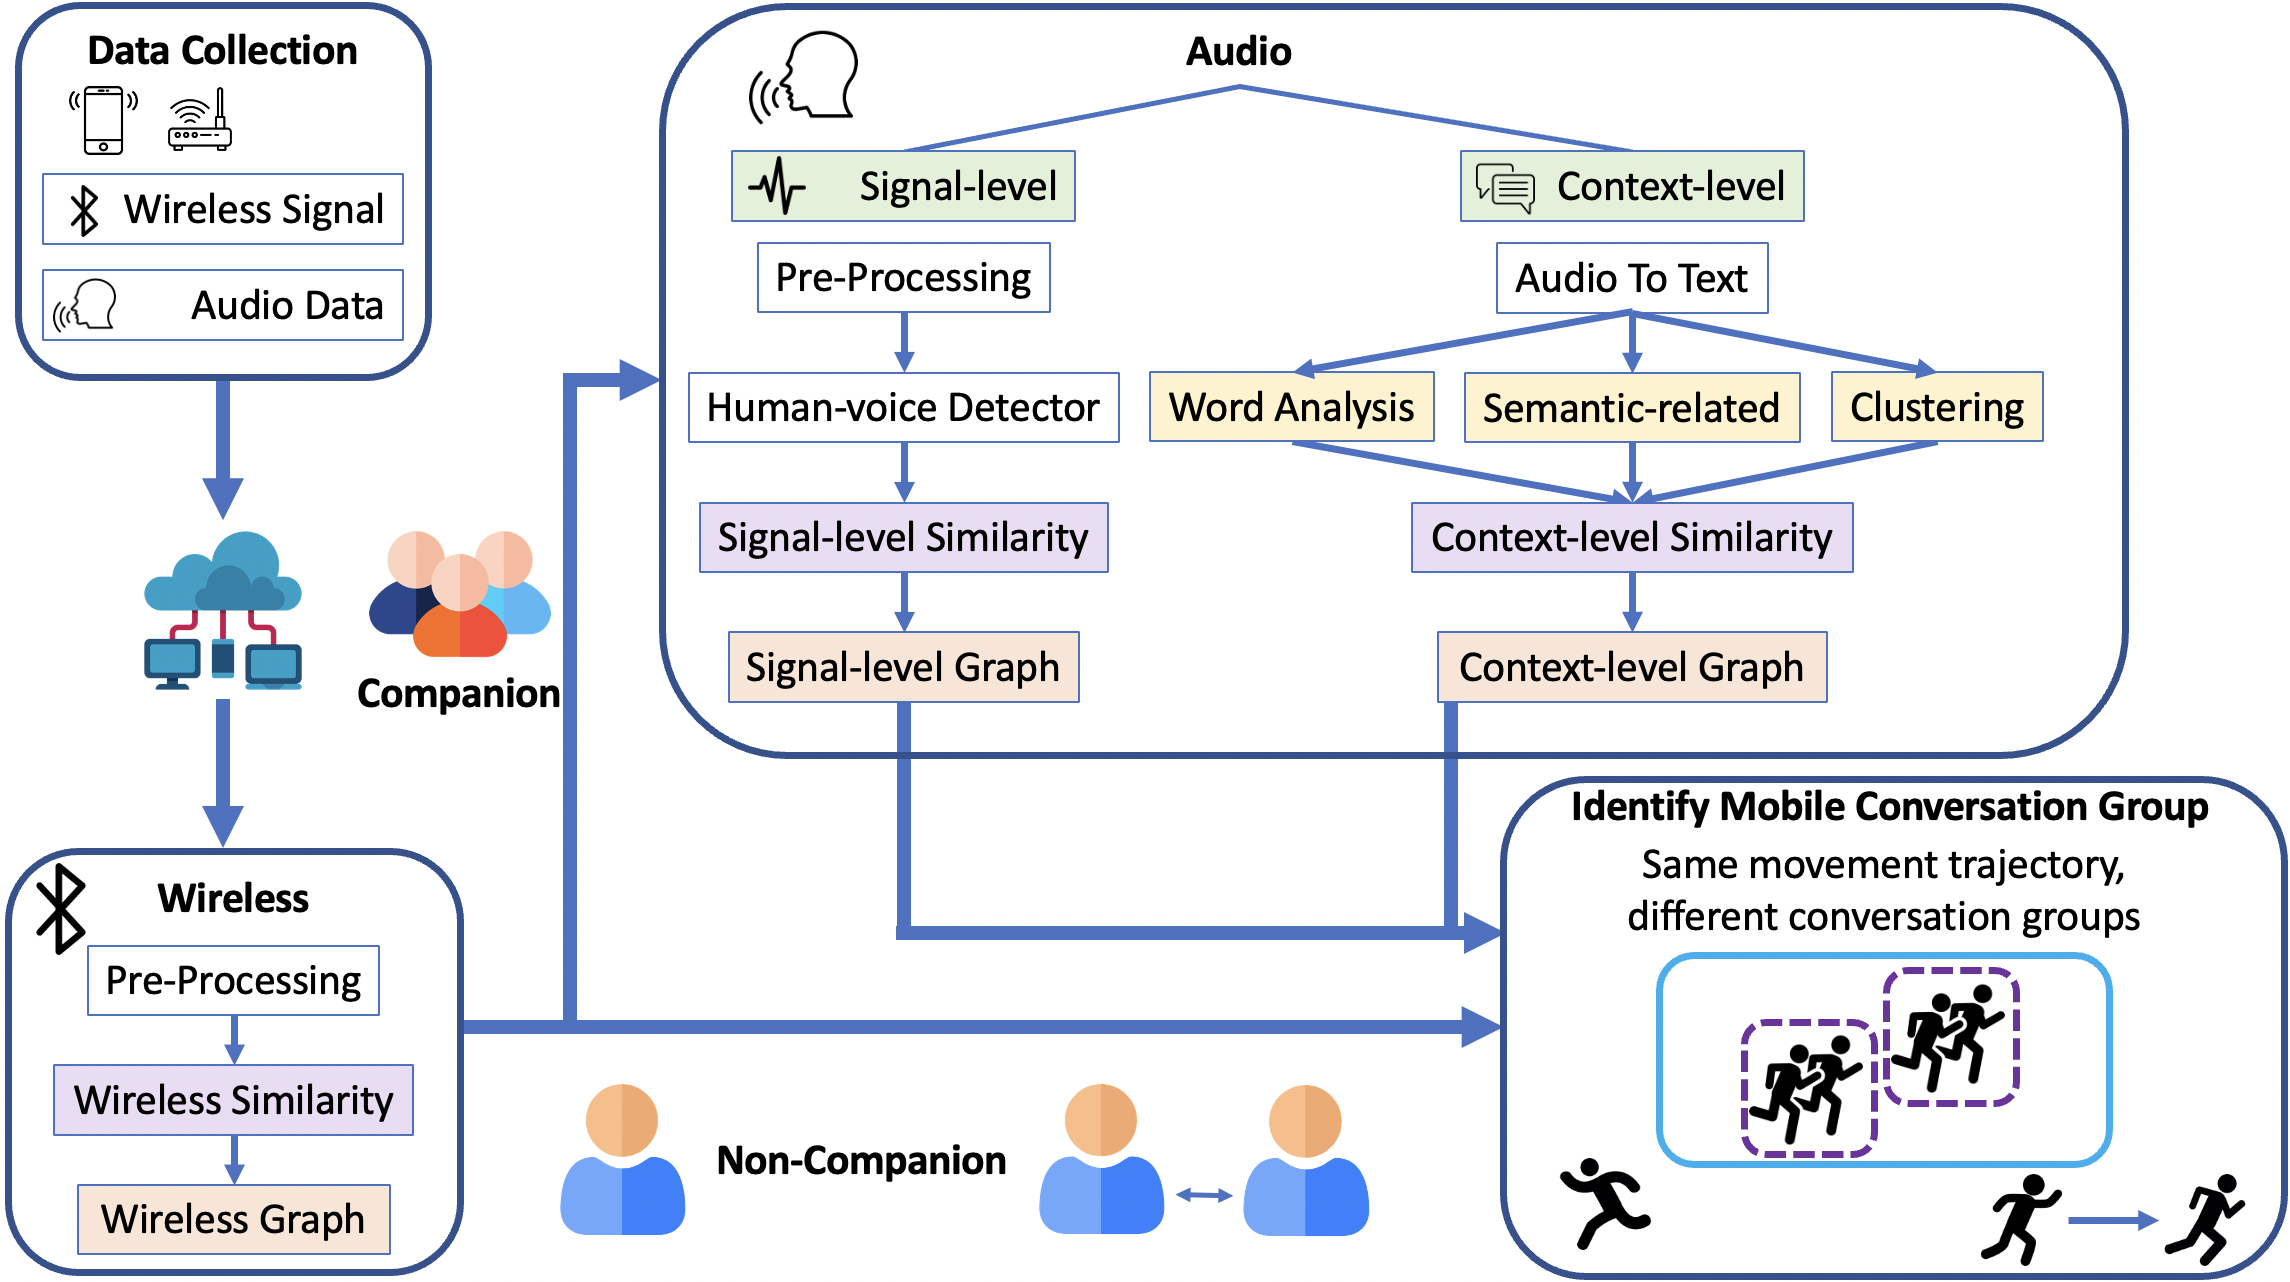
\includegraphics[width=6.3in,height=3.5in]{images and data/System_Architecture_Yun.png}
\caption{System architecture of proposed method, which consists of the hybrid of wireless signal and audio features and recognition mobility and conversation groups.}
\label{f:system_model}
\end{center}
\end{figure}
%=== figure === %
%*----------Wireless Signal Start------------
\section{Wireless Signal}
\paragraph{}
Through the sniffers composed of Raspberry Pi, the wireless signal data of each mobile phone device can be obtained. At this stage, the processing method of \cite{chen2019witrack} is used. The Raspberry Pi records the timestamp, the UUID of the device, and the RSSI strength value. With the above data, we can analyze the wireless signal. The following are the general steps: Resample -> Normalize -> Smooth -> Calculate Similarity -> Detect Community. From Resample to Calculate Similarity are all methods (Reference: Senior), you can also refer to the method of \cite{lai2021viwise} \cite{tsai2020proximity} to get the similarity between the two devices, and then use our method to Detect Community.
%--
\\
\\
\textbf{Resample.} For the collected data, each mobile phone takes out the maximum RSSI strength value for each sniffer every second and resamples it into only one data of the mobile phone per sniffer per second.

\textbf{Normalize.} Use the min-max normalization method to normalize our data for subsequent analysis.

\textbf{Smooth.} Use Simple Exponential Smoothing Filter (SESF) and Savitzky-Golay (SAVGOL) Filter to smooth the RSSI curve.

\textbf{Calculate Similarity.} We use cosine similarity to calculate the movement trajectory similarity between the two devices. If the movement trajectory between the two devices is similar, a larger similarity value can be obtained in this step; otherwise, the opposite is true.

\textbf{Detect Community.} With the similarity value of the previous step, we can consider each device as a node on a graph, and the similarity is the weight of the edge between the two devices. With the graph, we use Louvain's Algorithm to help us find out the group relationship. In our dataset, the resolution parameter of 0.7 can accurately distinguish the three-movement relationships of emph{Companion}, emph{Leader-Follower} and emph{Independent}.
%*----------Wireless Signal End------------
%*----------Audio Feature Start------------
\section{Audio Feature}
\paragraph{}
In the audio feature part, we start the analysis from two aspects: Signal and Context, both of which can be carried out independently, and can have their own grouping results in both aspects.
%*---------Signal-level Start---------
\subsection{Signal-level}
\paragraph{}
In this part, we want to find out the time point when each person speaks. Because theoretically if they are in the same conversation group, the conversation between two people should be back and forth. If the time points that the two people's speech of the overlapping rate is low, it means that the two people are more likely to be in the same conversation group; and if the overlapping rate of time points between two people is high, it may be a different group of people. So they are talking at the same time. We designed a detector that can effectively distinguish conversation groups after a series of analyses of speech signals. The design method of the detector is roughly as follows: Remove Noise -> Take Absolute Value -> Normalize -> Set Parameter -> Calculate Similarity. The first three steps are all data pre-processing stages.
%--
\paragraph{}
We use the python library 'noisereduce' to help us to remove the noise of the signals, and the version of the library is 2.0.1. After this stage of processing, it can help us effectively reduce the ambient sound, leaving only the voice of the person we need.
\\
Because we just want to explore whether the user is speaking or not, we only need to consider the amplitude of the sound wave in the part of the signal wave, and the waveform is not what we want to discuss. So after removing the noise, we will take the absolute value of all the signals. The larger the absolute value is, the larger the amplitude is, and the more it represents the voice signal of the user speaking.
\\
There are individual differences in the volume of people's voices, and the brands and models of recording devices (smartphones) are inconsistent, so the data needs to be processed by normalizing. After removing the noise and taking the absolute value, we use the min-max normalization method to unify the scope of our data. In our study, we normalize the data to 0 $\sim$ 1000.
%--
\paragraph{}
The above are all stages of data pre-processing, and then the analysis of the time point of the user's speech must be started. We design a threshold-based human-voice detector. It is used to detect whether the user is speaking or not at a specific time point. Here's our design approach. We set three parameters by ourselves, namely: \textbf{Voice-Threshold}, \textbf{Time-Period}, and \textbf{Percent-Threshold}. Voice-Threshold means that if the value exceeds this value, it will be regarded as a human voice. With this parameter, the subtle ambient sound can be filtered again. Time-Period is a time interval, which can be 1 second, 0.5 seconds, or a smaller time unit. Percent-Threshold is the proportion. Combining these three parameters: If in Time-Period, there are more data points than Percent-Threshold ratio greater than Voice-Threshold, it is considered that the user is speaking. If 'Speaking', marked as 1; otherwise, marked as 0. So each user gets an array of 0s and 1s. Example: If the array calculated by a user is [0, 0, 1, 1, 0, 0, 1, 1, 0, 0], it means that the user is speaking at the third, fourth, seventh and eighth time points.
%--
\paragraph{}
With the array calculated by each user, we can use the Hamming Distance to calculate the similarity between the two users. If the Hamming Distance is larger, it means that the two users are speaking at the time. The more divergent it is, the more likely they are in the same conversation group. Because when two people are talking, there will theoretically be a time series relationship without overlapping. When the Hamming Distance is smaller, it means that there is a high degree of overlap at the speaking time point, and there is a lower possibility of being in the same conversation group. The calculated Hamming Distance value is \emph{signal-level similarity}.
%--
\paragraph{}
If you want to have a grouping result at this stage, you can use Louvain's Algorithm to help us find out the group relationship: Consider each user as a node on the graph, and the Hamming Distance between the two is the weight on the edge. With these values, the conversation group can be found. Or it can be used with the grouping results of the context-level section (please refer to the next section for details) to make the final grouping judgment.
%*---------Signal-level End---------
%*---------Context-level Start---------
\subsection{Context-level}
\paragraph{}
In this analysis phase, we analyze the content of the conversation. After collecting the audio data, the voice file will be converted into a text file first. We will analyze the text in three aspects: \emph{Word Analysis}, \emph{Semantic-related Analysis} and \emph{Density/Centroid-based Clustering}. After linear integration of these three aspects, we can find out the conversation group to achieve our goal. The three aspects are described in detail below:
%--
\paragraph{}
\textbf{Word Analysis.} We want to know if two people are talking about repeated words, so we analyze the words that appear. In this part, simply calculate the content of the two people's speech and whether there are repeated words. After converting the user's recording file into text, it will be subdivided into two methods: \emph{With stop words} and \emph{Without stop words}. In \emph{With stop words}, we directly calculate the similarity of the words appearing in the text files of the two users; and in \emph{Without stop words}, we first remove the stop word, and then calculate the similarity. For the calculation of similarity, we choose two of methods in \cite{9198782}, (\ref{e:similarity1}) and (\ref{e:similarity2}), where $T_1$ and $T_2$ are the sets of words that appear in the two users respectively. With two pre-processing methods (with or without stop words) and two similarity calculation methods (\ref{e:similarity1} and \ref{e:similarity2}), there are four values for every two people. After averaging the four values, this is the Normalized Similarity for this aspect.
\\

% \begin{equation}
% \label{e:similarity1}
% Similarity1=\frac{|T_1\cap T_2 |}{Max(|T_1|,|T_2|)}\; (Braun\frac{\;}{\;}Blanquet\;Similarity)
% \end{equation}
% %--
% \begin{equation}
% \label{e:similarity2}
% Similarity2=2 \times \frac{|T_1\cap T_2 |}{|T_1|+|T_2|}\;(Dice\;Similarity)
% \end{equation}


\begin{alignat}{2}
&Similarity1=\frac{|T_1\cap T_2 |}{Max(|T_1|,|T_2|)}\; &(Braun\frac{\;}{\;}Blanquet\;Similarity) 
\label{e:similarity1}\\  
 &Similarity2=2 \times \frac{|T_1\cap T_2 |}{|T_1|+|T_2|}\;&(Dice\;Similarity)
\label{e:similarity2}
\end{alignat}


%--
\paragraph{}
\textbf{Semantic-related Analysis}. In order to understand the people, events, time, place and objects that appear in the dialogue content, or even more detailed dialogue content. We use a python library: spaCy, to help us achieve this goal. The entity features in this library can help us find words in specific categories. We convert the number of categories and words found by the kit into a $1\times15$ -dimensional vector (15 is the total number of categories). Then calculate the inner product of the two-person vectors. The purpose is to understand the distance relationship between two vectors in space. The closer the distance, the higher the inner product value, and the farther the distance, the lower the inner product value. Because the value after the inner product will theoretically not fall between 0 and 1. Therefore, we have to normalize the data after the inner product. The processed value is the \emph{Normalized Similarity} at this stage.
%--
\paragraph{}
\textbf{Density/Centroid-based Clustering}. In this part, we want to know if the conversation between two people revolves around the same theme. Sometimes talking about the same topic doesn't necessarily mean repeating the same words over and over again. To see if there is a theme around, we transform the words into a vector space. Words with similar meanings will be close together. We want to find keywords from it, so remove stop words first. Then, according to the frequency of word occurrence, select the top ten words that appear most frequently. For these ten words, the Word2Vec model is used to project them into the vector space. In the vector space, there is a concept of distance between each word, so words can be grouped. Words that are close in distance (that is, semantically similar) are classified into the same group. The clustering methods we use are DBSCAN and K-means. After grouping, some subgroups will have more words in them, while some will have fewer words, and even a single word is an individual subgroup. However, we found that the keywords related to the dialogue topic usually appear in the \emph{non-maximum subgroup}. Therefore, our analysis method will remove the largest(maximum number of words) subgroup and combine the words in other smaller subgroups, denoted as $T_n$. Then calculate the similarity between the two people. The calculation method is the same as (\ref{e:similarity1}) and (\ref{e:similarity2}). Two clustering methods (DBSCAN and K-means) are combined with two similarity calculation methods, and there are four values for every two people. After averaging the four values, this is the \emph{Normalized Similarity} for this aspect.

\paragraph{}
At this stage, in the K-means clustering method, our default parameter is to divide the words into three groups, that is, k=3. Because if it is only divided into two groups, after removing the subgroup with the largest number of words, there will be only one group left; if it is divided into four groups, after our research, we find that the effect is not as good as k=3, so k=3 is finally selected. In the grouping method of DBSCAN, eps=2.0 (the distance is regarded as the same group) and min-samples=1 (at least a few points in a group), the above are the results of our experiments.
%--
\\
\\
\textbf{Context-level Similarity}.\\
Context-level contains three oriented analyses. By integrating the three oriented results (\emph{Normalized Similarity}), it can be judged whether the two are the same conversation group. Here's how to integrate by linear combination:
% $$Normalized\;Similarity(in\;Word\;Analysis)\times \alpha +$$\\
% $$Normalized\;Similarity(in\;Semantic-related\;Analysis)\times \beta +$$\\
% $$Normalized\;Similarity(in\;Density/Centroid-based\;Clustering )\times \gamma$$\\
% $$=Final Value$$

\begin{equation*}%加*表示不對公式編號
\begin{split}
&Normalized\;Similarity(in\;Word\;Analysis)\times \alpha +\\
&Normalized\;Similarity(in\;Semantic\frac{\;}{\;}related\;Analysis)\times \beta +\\
&Normalized\;Similarity(in\;Density/Centroid\frac{\;}{\;}based\;Clustering )\times \gamma\\
&=Context\frac{\;}{\;}level\;Similarity\\
&,and\quad\alpha+ \beta+ \gamma=1
\end{split}
\end{equation*}
\\
% And $\alpha+ \beta+ \gamma=1$.
When the weights of $\alpha$, $\beta$ and $\gamma$ are determined. There is a unique \emph{Context-level Similarity} between every two users, which is the similarity of the \textbf{Context-level}. After averaging these \emph{Context-level Similarity} (6 in our experiment), it is the \textbf{Threshold} under this weight. If the \emph{Context-level Similarity} of the combination $\geq$ \textbf{Threshold}, it is regarded as the same conversation group, otherwise, it is a different conversation group.

%*---------Context-level End---------
%*---------Integration Start---------
\subsection{Integration of Signal-level and Context-level}
\paragraph{}
At \textbf{Signal-level} and \textbf{Context-level}, there is an independent similarity value between every two people. They are represented as $S_n$ and $C_n$, respectively, where $n$ is an integer, representing a combination of two people as a group. For example, User A and User B are the first group combination, then the similarity between User A and User B is $S_1$ and $C_1$. After re-specifying the value of similarity using the following formula:

\begin{equation*}%加*表示不對公式編號
\begin{split}
S_n=\begin{cases}S_n&,if\,S_n\,is\,regarded\,as\,the\,same\,group
 \\
S_n\times(-1)&,otherwise
\end{cases}
\end{split}
\end{equation*}

\begin{equation*}%加*表示不對公式編號
\begin{split}
C_n=\begin{cases}C_n&,if\,C_n\,is\,regarded\,as\,the\,same\,group
 \\
C_n\times(-1)&,otherwise
\end{cases}
\end{split}
\end{equation*}


Considering each user as a node, there is an edge between every two users, and $S_n$ and $C_n$ are the weights on the edge. In this way, the relationship diagrams at the Signal-level and Context-level can be generated respectively. After adding the weights on the two graphs, if the weights on the edges are greater than or equal to 0, then the two are the same conversation group; otherwise, the combination is a different conversation group. The schematic diagram is shown in Figure \ref{f:System_Design_Integration_SandC}. Four different color nodes represent four different users.
\\
%=== figure === %
\begin{figure}[btph]
\begin{center}
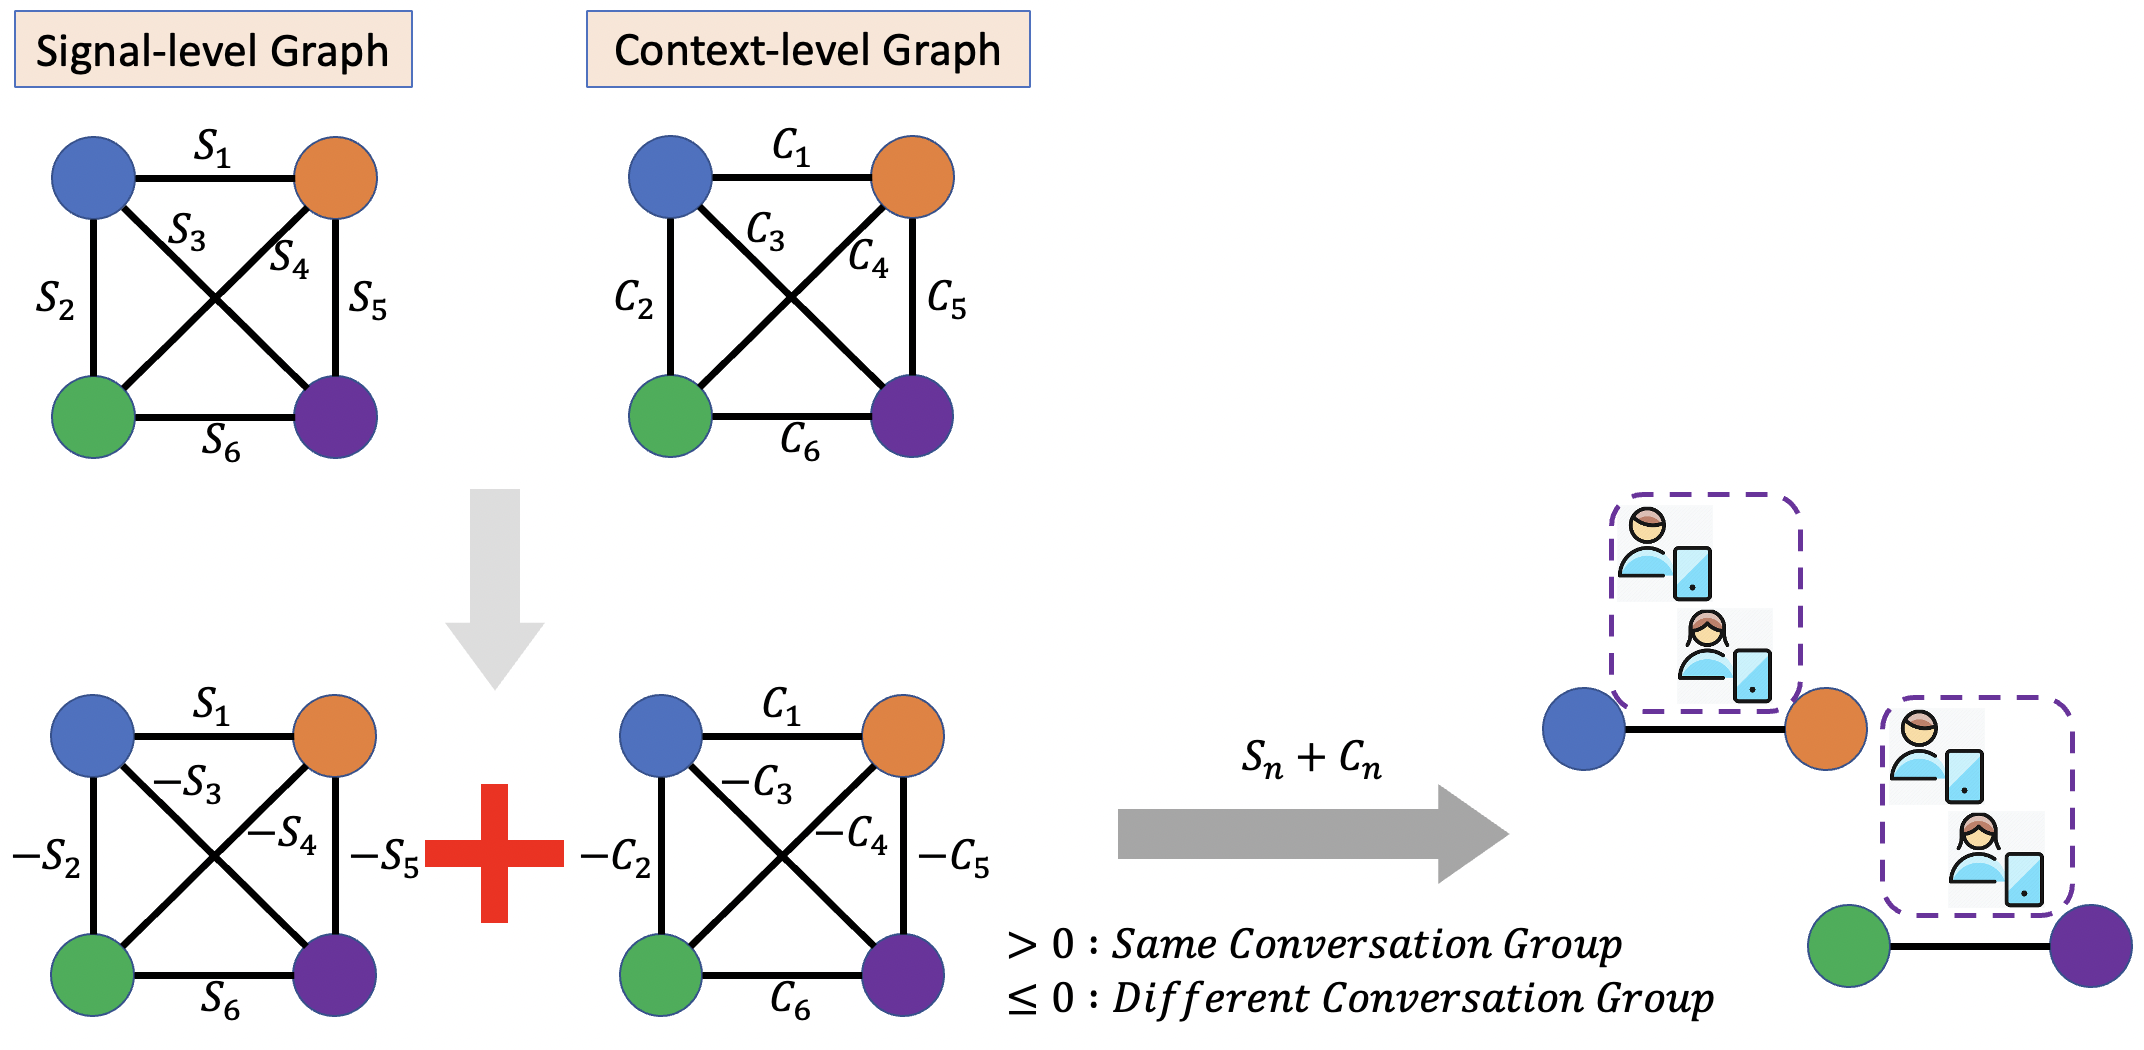
\includegraphics[width=6.3in,height=3in]{images and data/System_Integration_SandC_Yun.png}
%2.1:1
\caption{The method of integration of Signal-level and Context-level}
\label{f:System_Design_Integration_SandC}
\end{center}
\end{figure}
%=== figure === %
\\
The above is a partial analysis of audio, with the non-companion relationship distinguished from the wireless signal part, it can be applied to many practical examples.
%*---------Integration End---------
%*----------Audio Feature End------------
%*---------------------System Design End---------------------------------

%*-------------------Experimental Setup Start------------------------------
\chapter{Experimental Setup}
%*----------Mobile Relationship Setup Start---------
\section{Mobile Relationship Setup}
\paragraph{}
In our study, a total of seven participants were assigned to three mobile social relationships: \emph{Companion}, \emph{Leader-Follower}, and \emph{Independent}. Four of them are in a \emph{Companion} relationship, that is, they are the same on the moving trajectory; two of them are in a \emph{Leader-Follower} relationship, one walks ahead, and the other keeps a certain distance behind; the remaining is \emph{Independent} and has the characteristic of walking around at will. The people assigned to \emph{Companion} will move together and have conversations, in the conversation section there is a limit of two conversation groups, meaning two of them to talk about a topic with each other, and the other two talk about another completely unrelated thing. There will be no verbal communication between the two groups of people, it is simply two groups of people walking together, talking about different topics; and \emph{Leader-Follower} relationship will maintain a distance between the front and rear, so there will be no conversational communication; \emph{Independent} relationship will not have any voice interaction with anyone because it moves around at will.
%*----------Mobile Relationship Setup End---------
%*----------Experiment Environment Start---------
\section{Experiment Environment}
\paragraph{}
The main experimental environment is located on the fifth floor of the Electrical Engineering Department of our school (National Cheng Kung University). Part of the corridor on this floor is where we collect experimental data. The experimental route is a T-shape, as shown in Figure \ref{f:Experimental_Setup_Map} . The corridor is 2.4 meters wide, one section is 37.6 meters long, and the other section is 33.2 meters long.
%=== figure === %
\begin{figure}[btph]
\begin{center}
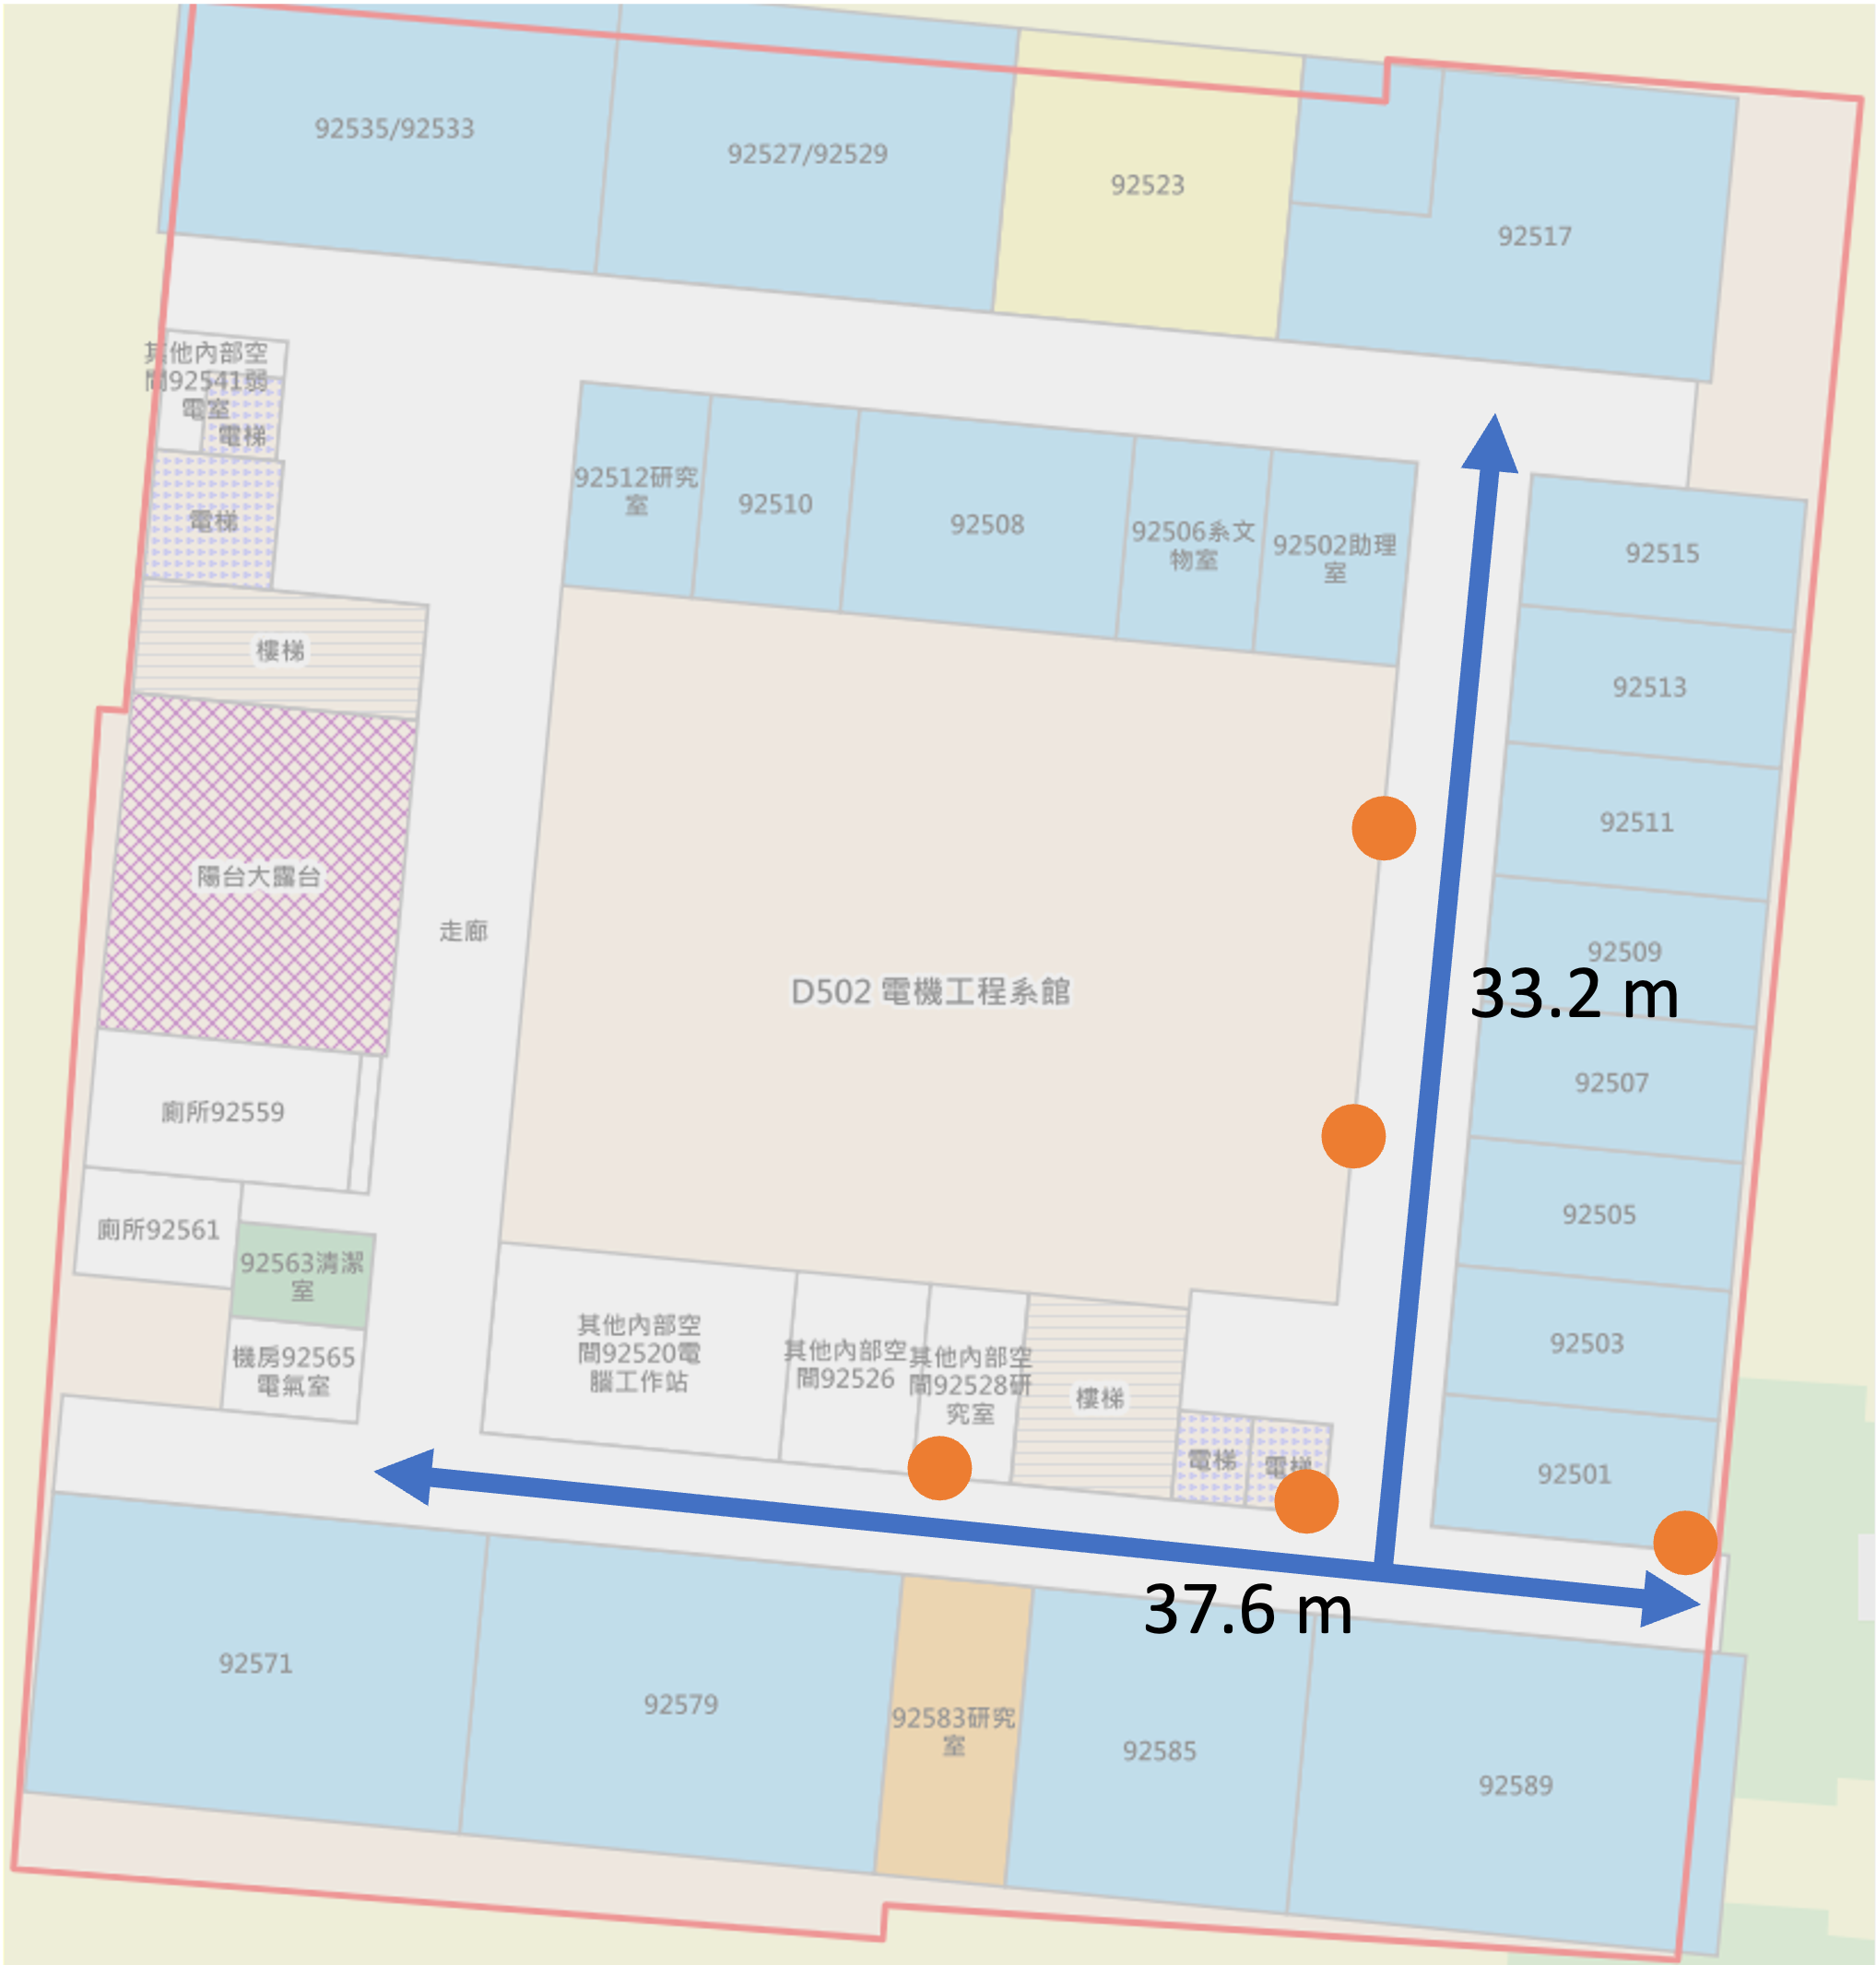
\includegraphics[width=4in,height=4.2in]{images and data/Experimental_Setup_Map_Yun.png}
%width=6.1 height=6.4
\caption{Experiment Environment : The blue line segments are the walking routes, and the orange points are the positions of the sniffers}
\label{f:Experimental_Setup_Map}
\end{center}
\end{figure}
%=== figure === %
%*----------Experiment Environment End---------
%*----------Data Collection Start---------
%=== figure === %
\begin{figure}[btph]
\begin{center}
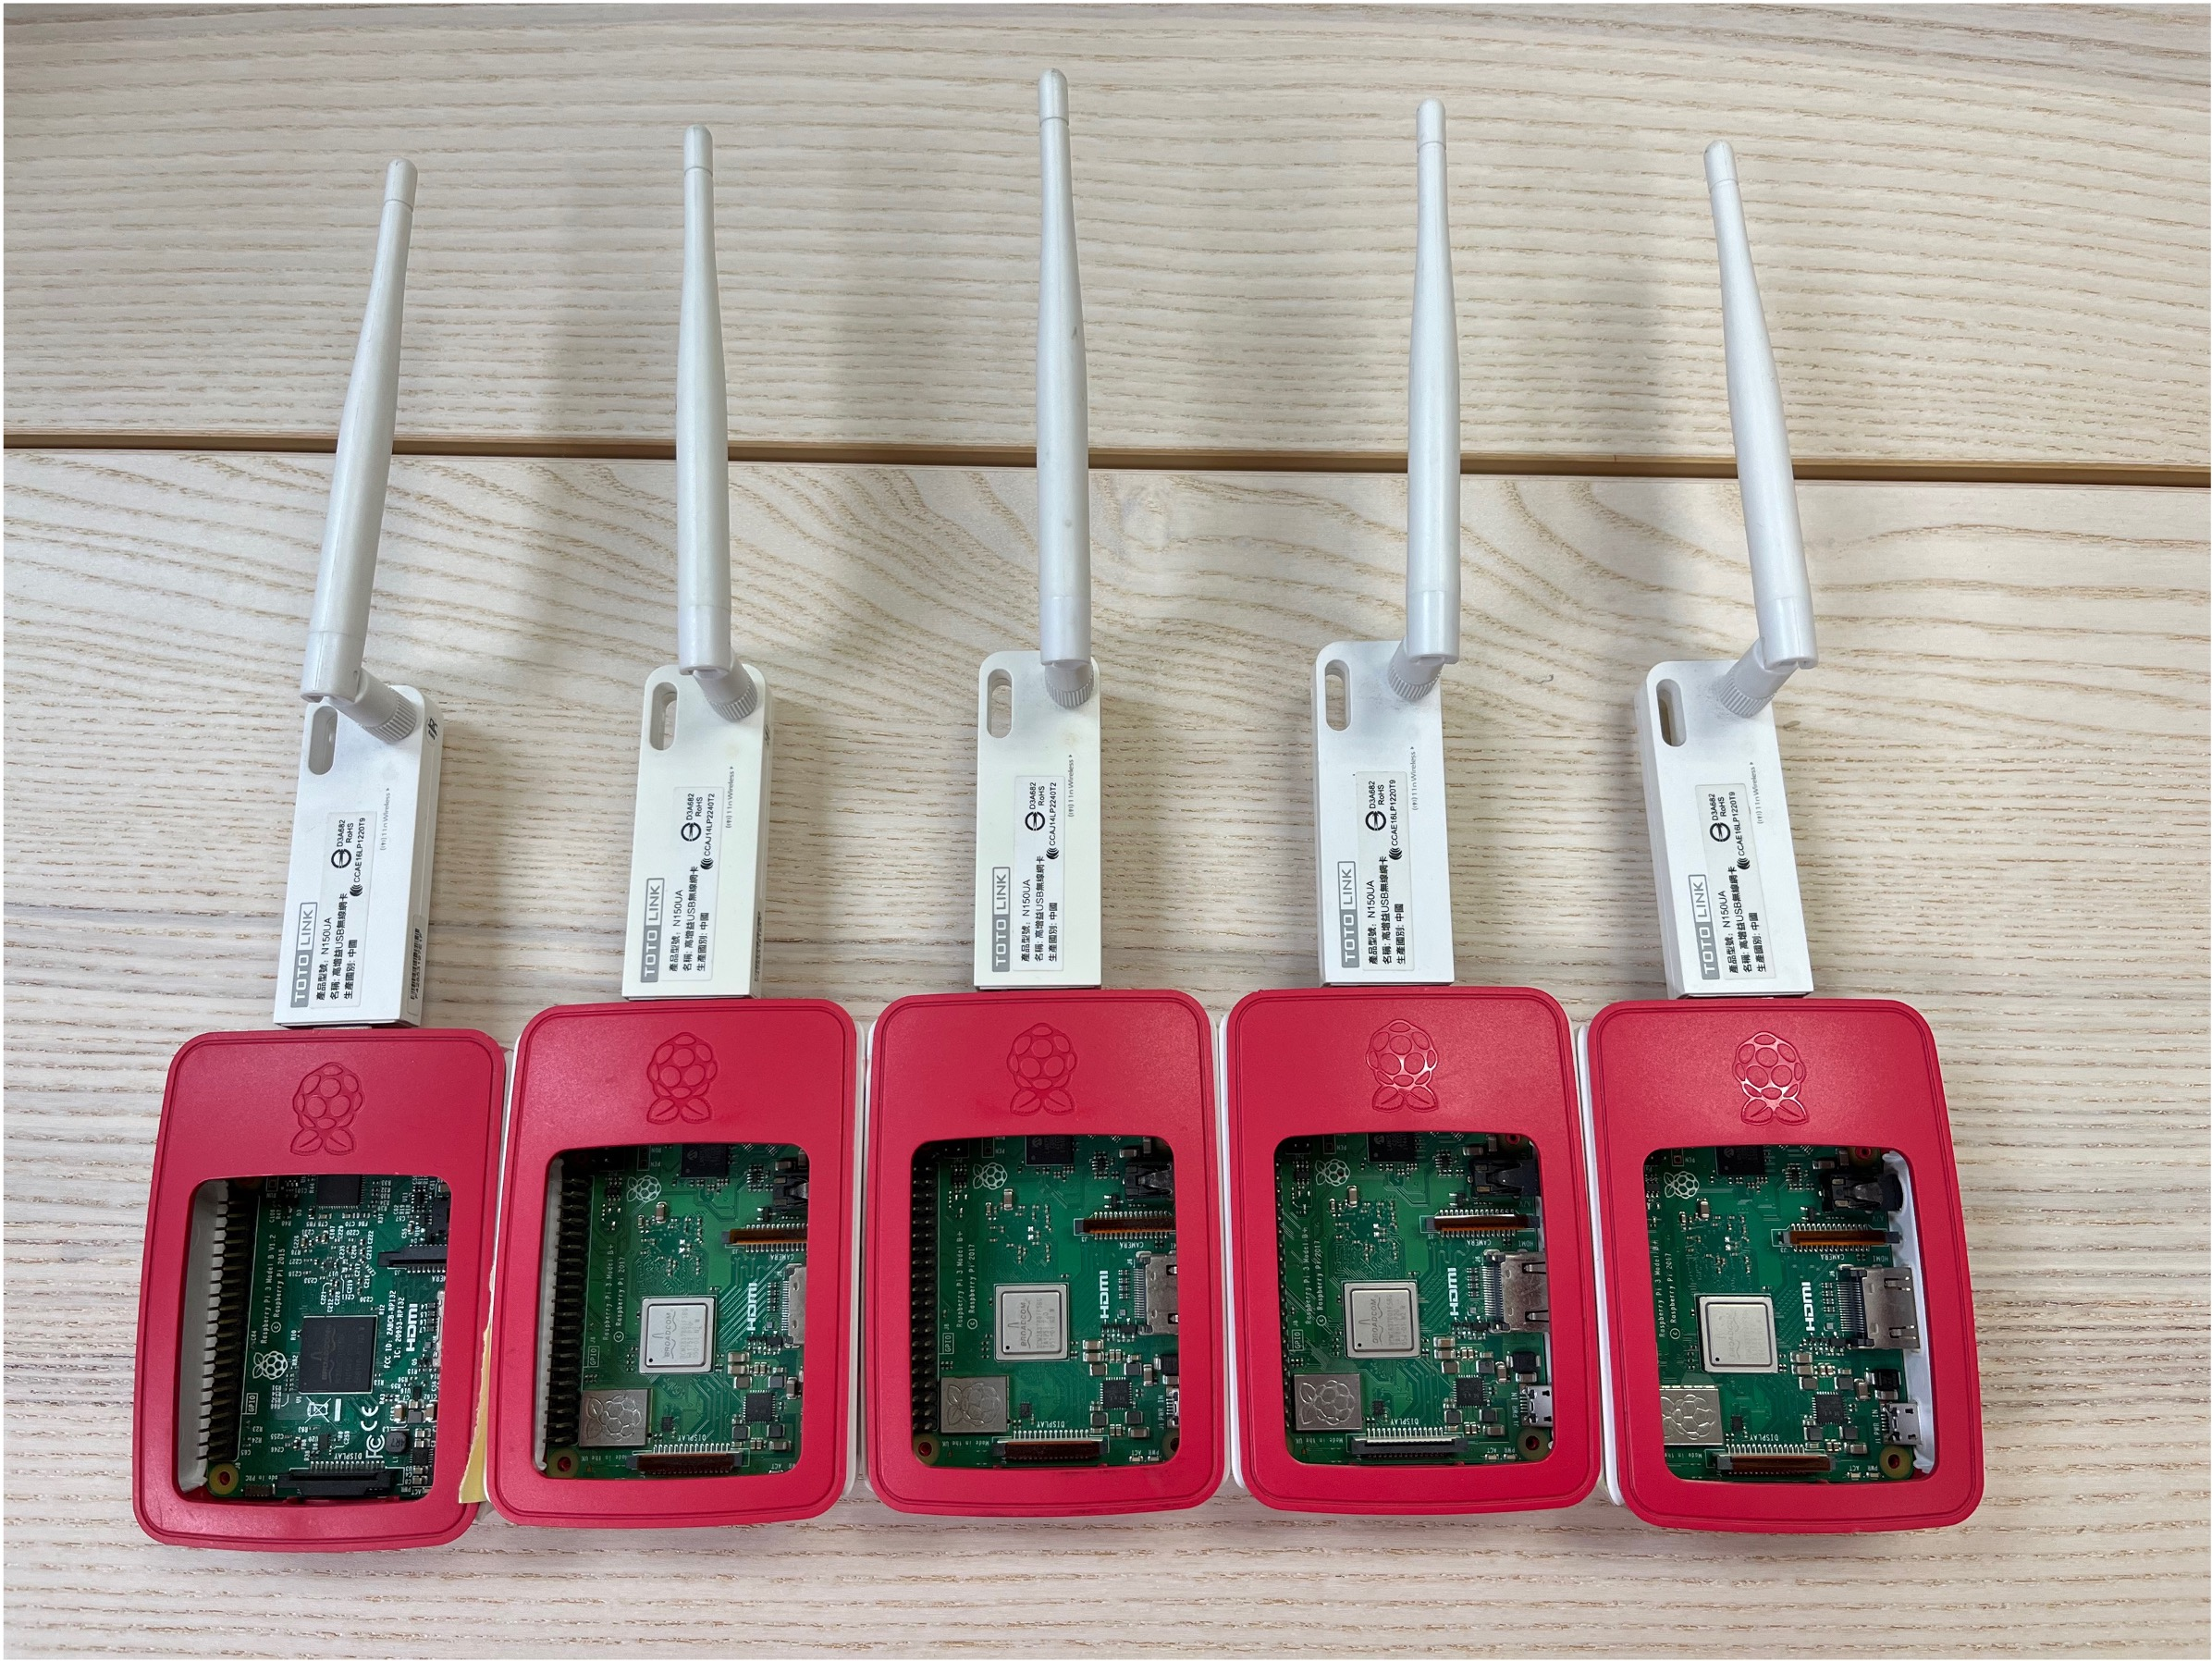
\includegraphics[width=4.66in,height=3.5in]{images and data/Experimental_Setup_Sniffers_Yun.jpg}
%width=7.2 height=5.4
\caption{Sniffers : Five Raspberry Pi 3B+ boards}
\label{f:Experimental_Setup_Sniffers}
\end{center}
\end{figure}
%=== figure === %
\section{Data Collection}
\paragraph{}
In the corridor of the experimental environment, a total of five sniffers are arranged. In our experiment, the Raspberry Pi 3B+ board is used as the sniffer (as shown in the Figure \ref{f:Experimental_Setup_Sniffers}). The function of the sniffers is to receive BLE signals from nearby devices. We use the signal strength to analyze the spatial information. The sniffers will be placed in the corridor of the experimental environment, 0.7 meters above the ground, and the sniffers are 1.2 meters apart.

\paragraph{}
All seven participants wore a smartphone as the experimental device. The mobile phone models are hTC UUltra, SHARP AQUOS V, Samsung A51, Moto G, hTC U11 and hTC U19e, as in Fig.\ref{f:Experimental_Setup_Devices}. In addition to sending BLE packets for the Raspberry Pi to receive, the function also collects voice data. We use the \emph{Easy Voice Recorder} app to help us record, through which we can do further voice analysis. During the recording process, the subjects will be given voice scripts and let them have a dialogue according to the scripts. The source of the script is Interactive Online Video Learning System from NCKU (National Cheng Kung University). The topics of the dialogue include Workplace, Daily Life, Cultural Differences, Health, Travel, Taiwan Features and Traffic, seven topics in total.

\paragraph{}
Arrange the sniffers in the corridor and the participants wear the experimental device (smartphone), then the experimental data can be collected. The subjects will move freely in the specified corridor area. The movement trajectories of the participants must be carried out according to the set. In the \emph{Companion} relationship, the dialogue script needs to be read while moving, so as to analyze the voice dialogue. The experimental scenario is shown in the Figure \ref{f:Experimental_Setup_Scenario}.
%=== figure === %
\begin{figure}[btph]
\begin{center}
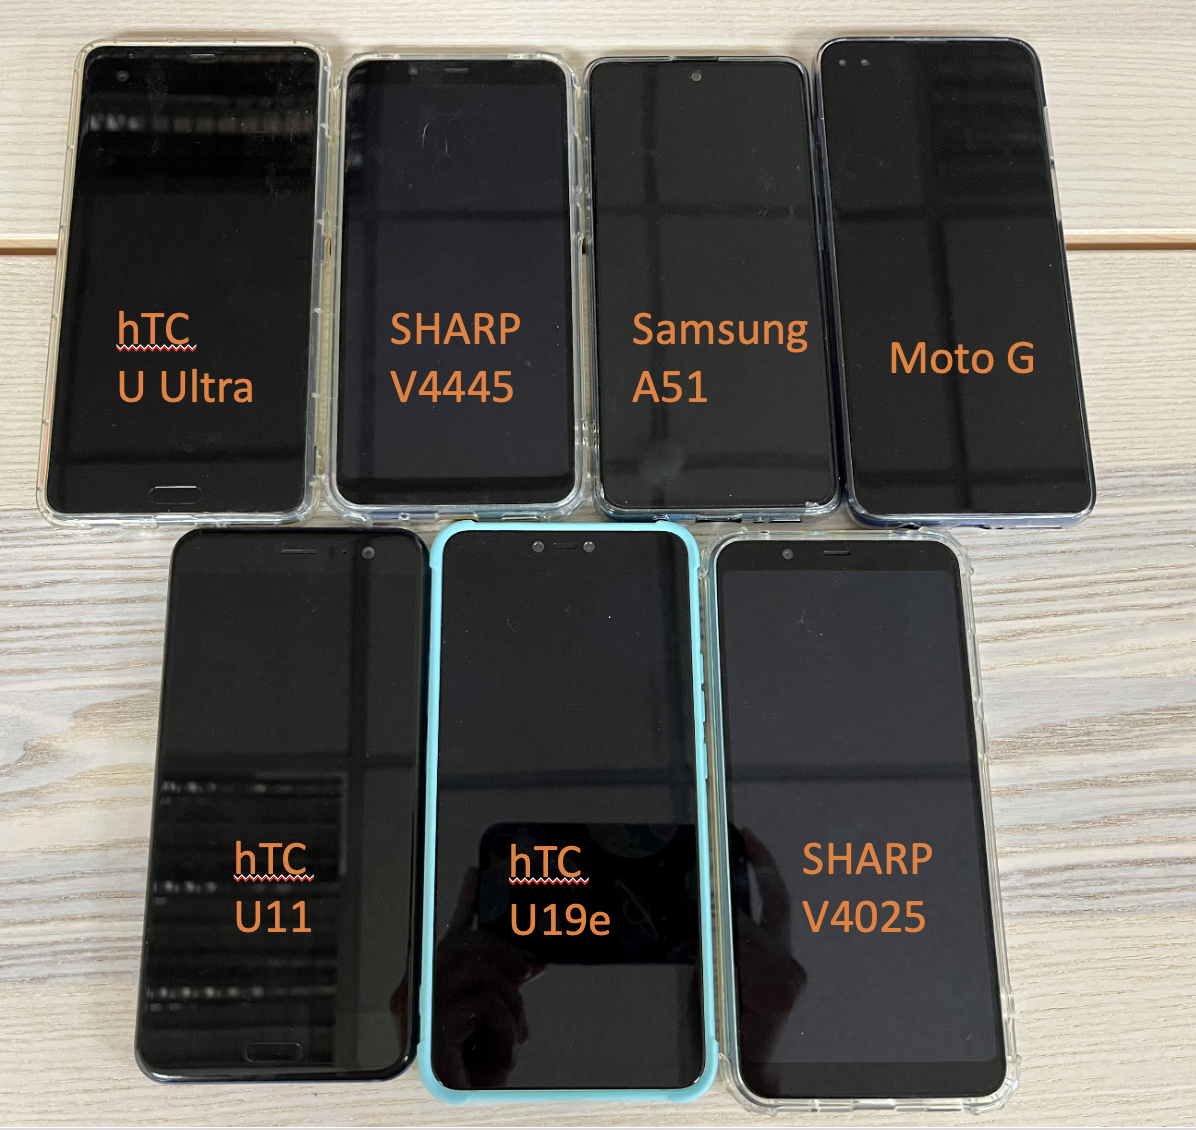
\includegraphics[width=4.25in,height=4in]{images and data/Experimental_Setup_Devices_Yun.png}
%width=6.9 height=6.5
\caption{Devices : Seven smartphones from different brands }
\label{f:Experimental_Setup_Devices}
\end{center}
\end{figure}
%=== figure === %
%=== figure === %
\begin{figure}[btph]
\begin{center}
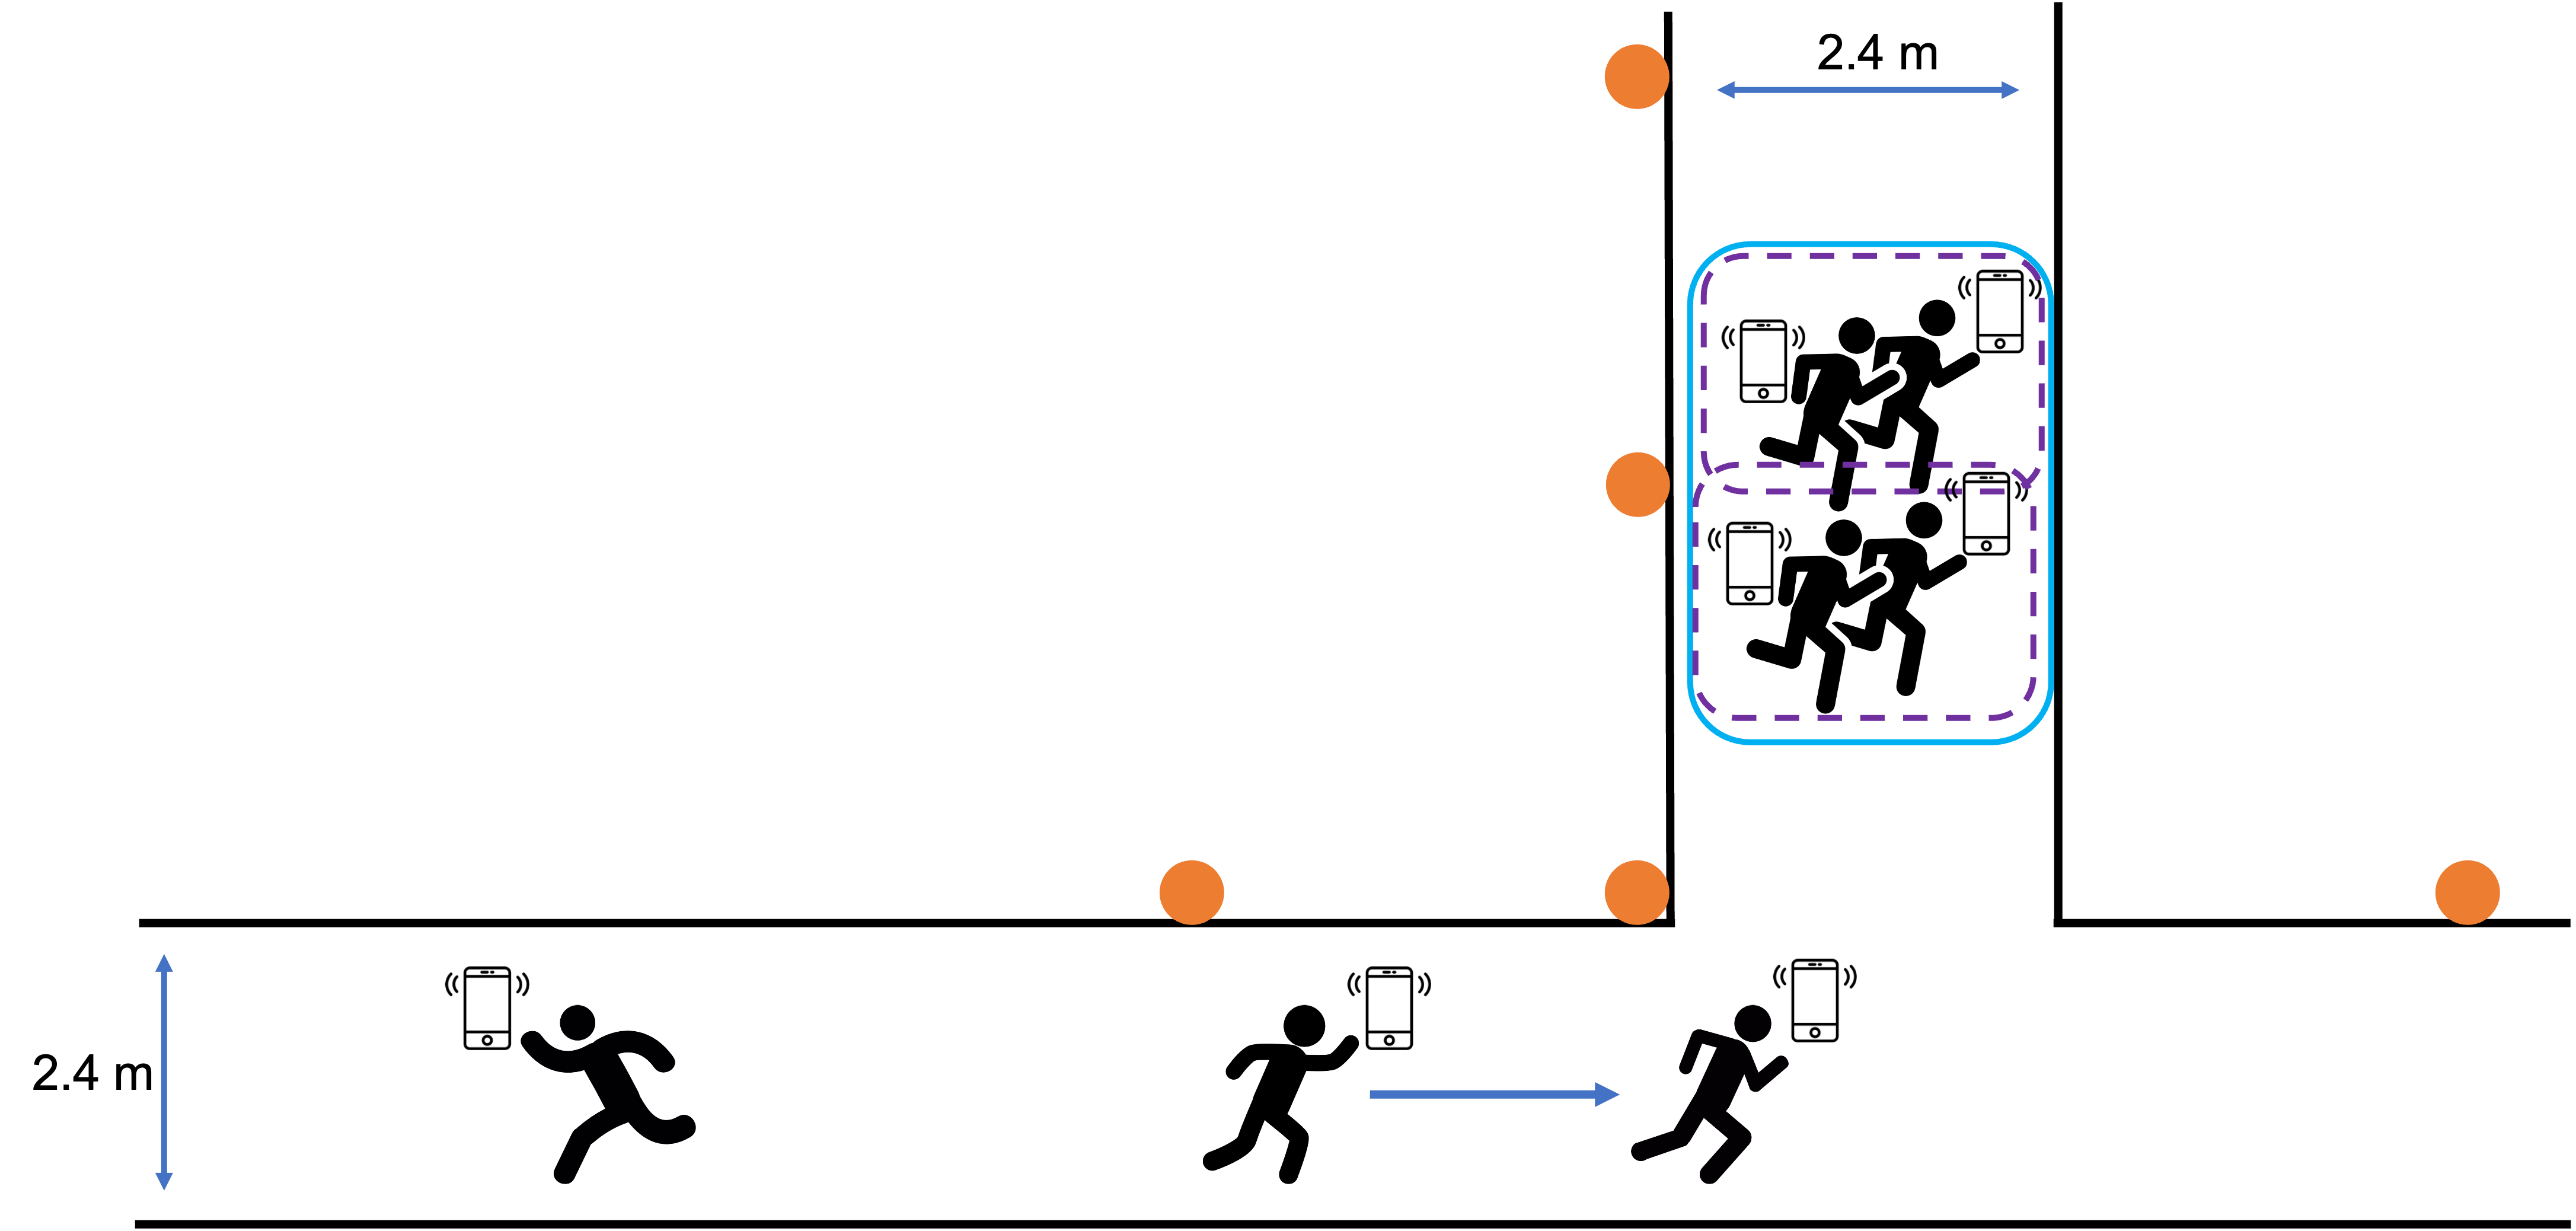
\includegraphics[width=6.3in,height=3in]{images and data/Experimental_Setup_Scenario_Yun.png}
% 2.1:1
\caption{Scenario (the orange points are the positions of the sniffers)}
\label{f:Experimental_Setup_Scenario}
\end{center}
\end{figure}
%=== figure === %
%*----------Data Collection End---------

%*-------------------Experimental Setup End------------------------------

%*-------------------Results Start--------------------------
\chapter{Results}
\paragraph{}
In this chapter, we will first compare our results with other similar papers, and then show the results of our research in each section.
%*-----------Comparing Performance Start---------
\section{Comparing Performance}
\paragraph{}
We choose to compare the results with the \cite{baker2017next2me}. Because in this paper, a combination of wireless and audio signals is used to analyze social conversation groups. It is very similar to our study.

% --table--
\begin{table}[btph]
\begin{center}
\caption{The result of the comparison with \cite{baker2017next2me}}
\label{t:Result_Comparision}
\begin{tabular}{|c|c|c|c|}
\hline
\textbf{Method} & \cite{baker2017next2me} -First Experiment     & \cite{baker2017next2me} -Second Experiment     & Proposed by us \\ \hline
\textbf{Accuracy(\%)} & 87.72 & 88  & 97.31 \\ \hline
\end{tabular}

\end{center}
\end{table}
% --table--

\paragraph{}
% In \cite{baker2017next2me}, the difference between Stage 1, 2, and 3 is the configuration of the number of people in each group. Hereinafter, Pn represents the number of the subject. In Stage 1, the author divided the seven people into three conversation groups. One group consisted of three persons (P1, P2, P3), and the other two groups consisted of two persons (P4, P5) (P6, P7); in Stage 2, seven subjects were divided into two groups, one group of four individuals (P1, P2, P6, P7), another group of three (P3, P4, P5); in Stage 3, the number of groups and the number of people in the group are the same as in Stage 1, but the subjects in the group are different combinations ( P3, P4, P5) (P1, P7) (P2, P6).

In this paper, we only take the audio analysis method, without the part of the wireless signal, and compare it with our method. We reproduce the analytical method \cite{baker2017next2me}. The data from our two experiments were applied to the method of \cite{baker2017next2me}.

\paragraph{}
As can be seen from Table \ref{t:Result_Comparision}, our results are better than that of the paper. Because we have considered and analyzed the content of the user's chat, not just from the signal part, to explore whether the user has spoken.
%*-----------Comparing Performance End---------
%*-----------Signal-level in Audio Feature Start---------
\section{Signal-level in Audio Feature}
\paragraph{}
In the Signal-level part, we designed a human-voice detector which is threshold-based. With the results of the detector, we use Louvain's Algorithm to help us cluster. We fixed the parameters of the detector and the algorithm, and the obtained clustering accuracy is \textbf{90\%}. With more subtle tweaks to the parameters, there is a chance to increase the accuracy to 100\% in each conversation. This result indicates that our approach for speech signals is feasible.

\paragraph{}
At this stage, the sampling rate of the audio signal is 16000Hz. The default parameters of our human-voice detector are followings : Voice-Threshold=75, Time-Period=0.25, Percent-Threshold=0.3. And in Louvain's Algorithm, resolution=1.4. The parameters of the human-voice detector can be modified due to different experimental data.

%*-----------Signal-level in Audio Feature End---------
%*-----------Context-level in Audio Feature Start---------
\section{Context-level in Audio Feature}
\subsection{Clustering Result Accuracy}
% --table--
\begin{table}[btph]
\begin{center}
\caption{The result in Context-level Similarity}
\label{t:Result_Context_Similarity}
\begin{tabular}{|c|c|c|c|c|c|c|}
\hline
\textbf{Conversation} & 1     & 2  & 3   & 4  & 5  & Average \\ \hline
\textbf{Accuracy(\%)} & 97.46 & 100 & 94.68 & 99.31 & 91.44 & 96.57      \\ \hline
\end{tabular}

\end{center}
\end{table}
% --table--

\paragraph{}
Table \ref{t:Result_Context_Similarity} presents the clustering result accuracy purely at the context-level. The value of each dialogue is the average of two experiments, from which it can be found that the accuracy is more than 90\%, and the overall average is as high as 96.57\%. If only the audio content data analysis is used, it also has a good effect.
\clearpage
\paragraph{}
In the first conversation, the topics of the two groups of subjects are Workplace and Travel; the second conversation topics are Daily Life and Taiwan Features; the third conversation: Cultural Differences and Traffic; the fourth are Health and Daily Life; the fifth topics are Travel and Workplace.
% \clearpage
\paragraph{}
Tables \ref{t:ConfusionMatrixFirst}, \ref{t:ConfusionMatrixSecond} and \ref{t:ConfusionMatrixCombine} are the confusion matrices of the results of the first experiment, the second experiment and the integration of the two experiments at the context-level, respectively. In Table \ref{t:PrecisionRecallF1Score}, which shows three indicators of precision, recall and f1-score in evaluation systems, it can be found that our system has a good effect on the audio part.

%-- table--
\begin{table}[btph]
\begin{center}
\caption{The confusion matrix in first experiment}
\label{t:ConfusionMatrixFirst}
\begin{tabular}{llclcl}
 &  & \multicolumn{2}{l}{Predicted} \\
 & \multicolumn{1}{l|}{} & Same Group & Different Group \\ \cline{2-4} 
\multicolumn{1}{c}{Actual} & \multicolumn{1}{l|}{Same Group} & 315 & 45 \\
 & \multicolumn{1}{l|}{Different Group} & 23 & 697
\end{tabular}

\end{center}
\end{table}
%-- table--
%---

%-- table--
\begin{table}[btph]
\begin{center}
\caption{The confusion matrix in second experiment}
\label{t:ConfusionMatrixSecond}
\begin{tabular}{llclcl}
 &  & \multicolumn{2}{l}{Predicted} \\
 & \multicolumn{1}{l|}{} & Same Group & Different Group \\ \cline{2-4} 
\multicolumn{1}{c}{Actual} & \multicolumn{1}{l|}{Same Group} & 356 & 4 \\
 & \multicolumn{1}{l|}{Different Group} & 2 & 718
\end{tabular}

\end{center}
\end{table}
%-- table--
%---
%-- table--
\begin{table}[btph]
\begin{center}
\caption{The confusion matrix in two experiments}
\label{t:ConfusionMatrixCombine}
\begin{tabular}{llclcl}
 &  & \multicolumn{2}{l}{Predicted} \\
 & \multicolumn{1}{l|}{} & Same Group & Different Group \\ \cline{2-4} 
\multicolumn{1}{c}{Actual} & \multicolumn{1}{l|}{Same Group} & 671 & 49 \\
 & \multicolumn{1}{l|}{Different Group} & 25 & 1415
\end{tabular}

\end{center}
\end{table}
%-- table--
\clearpage
%---
\paragraph{}
From the data point of view, whether in precision, recall or f1-score, the results of the second experiment are the best. The value of the f1-score is as high as 99.16\%, approaching 100\%. Combining the data of the two experiments on the time series, the results show that the f1-score reaches 94.77\%. It shows that our method also has good results in the two experimental data.
%-- table--
\begin{table}[btph]
\begin{center}
\caption{The value of precision, recall and f1-score}
\label{t:PrecisionRecallF1Score}
\begin{tabular}{|l|c|c|c|}
\hline
 & First Experiment & Second Experiment & Two Experiments \\ \hline
\textbf{Precision(\%)} & 93.2 & 99.44 & 96.41 \\ \hline
\textbf{Recall(\%)} & 87.5 & 98.89 & 93.19 \\ \hline
\textbf{F1-Score(\%)} & 90.26 & 99.16 & 94.77 \\ \hline
\end{tabular}
\end{center}
\end{table}
%-- table--
\clearpage
%--
\subsection{Threshold Method}
\paragraph{}
We want to show that, in the context-level section, the threshold for clustering is averaged as a feasible approach. Therefore, we adjusted the three weight values of $\alpha$, $\beta$ and $\gamma$ to the maximum (0.8) respectively, as shown in the Figure \ref{f:Result_Threshold}.

%=== figure === %
\begin{figure}[btph]
\begin{center}
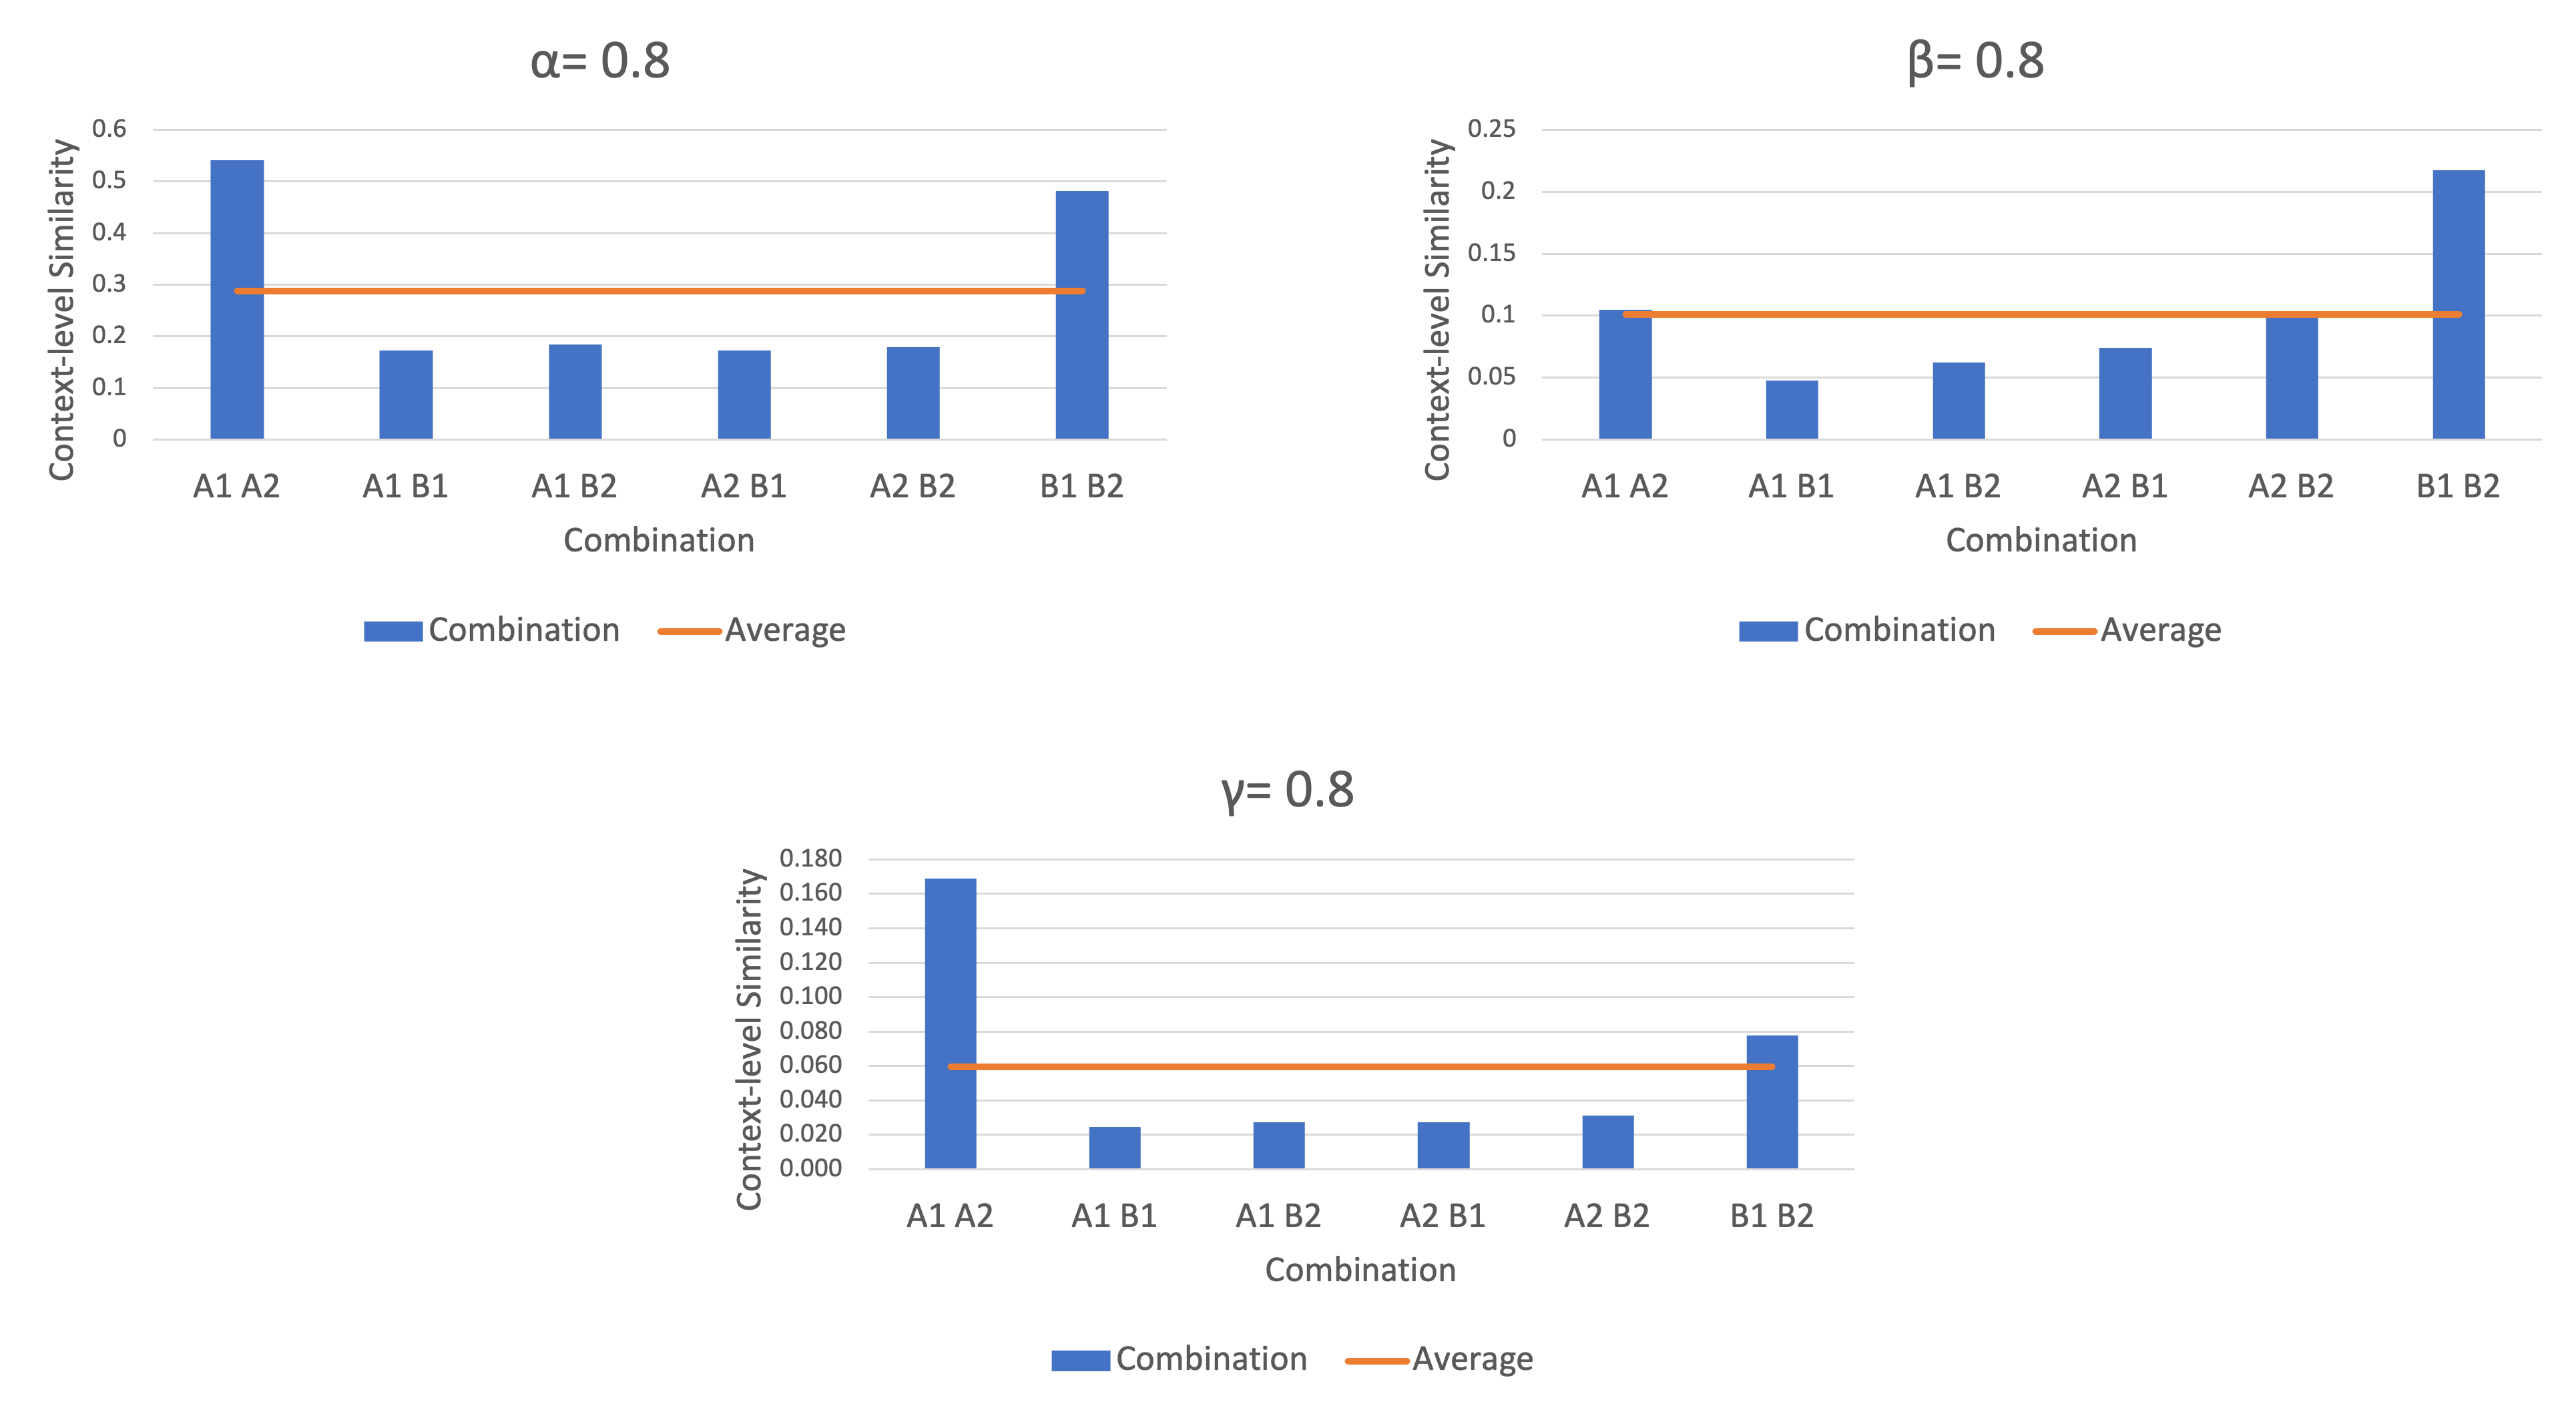
\includegraphics[width=6.41in,height=3.5in]{images and data/Result_Threshold.png}
% 1.83:1
\caption{Adjust all three weights to the maximum}
\label{f:Result_Threshold}
\end{center}
\end{figure}
%=== figure === %

\paragraph{}
In the three figures, the blue bars represent the calculated similarity between the two users. The orange horizontal line is the arithmetic mean of the bar chart values. It can be clearly seen that the similarity of the two combinations A1 A2 and B1 B2 (the same conversation group) is greater than the average; while the values of other user combinations (non-conversation groups) are all less than the average. Therefore, it can be seen that the selection method (average value) of the threshold value can effectively distinguish the conversation group.
\clearpage
%--
\subsection{The Effect of Weights}
\paragraph{}
At the Context-level, we use a linear combination approach to integrate the results from three different aspects (Word Analysis, Sematic-related Analysis, and Density/Centroid-based Clustering). In the Figure \ref{f:Result_Weight_Influence} there are four subplots. The two subgraphs in the upper half are the result graphs of two groups of users of the same conversation group under different linear combination weights. The subgraph in the lower half is a combination of two of the different groups.
%=== figure === %
\begin{figure}[btph]
\begin{center}
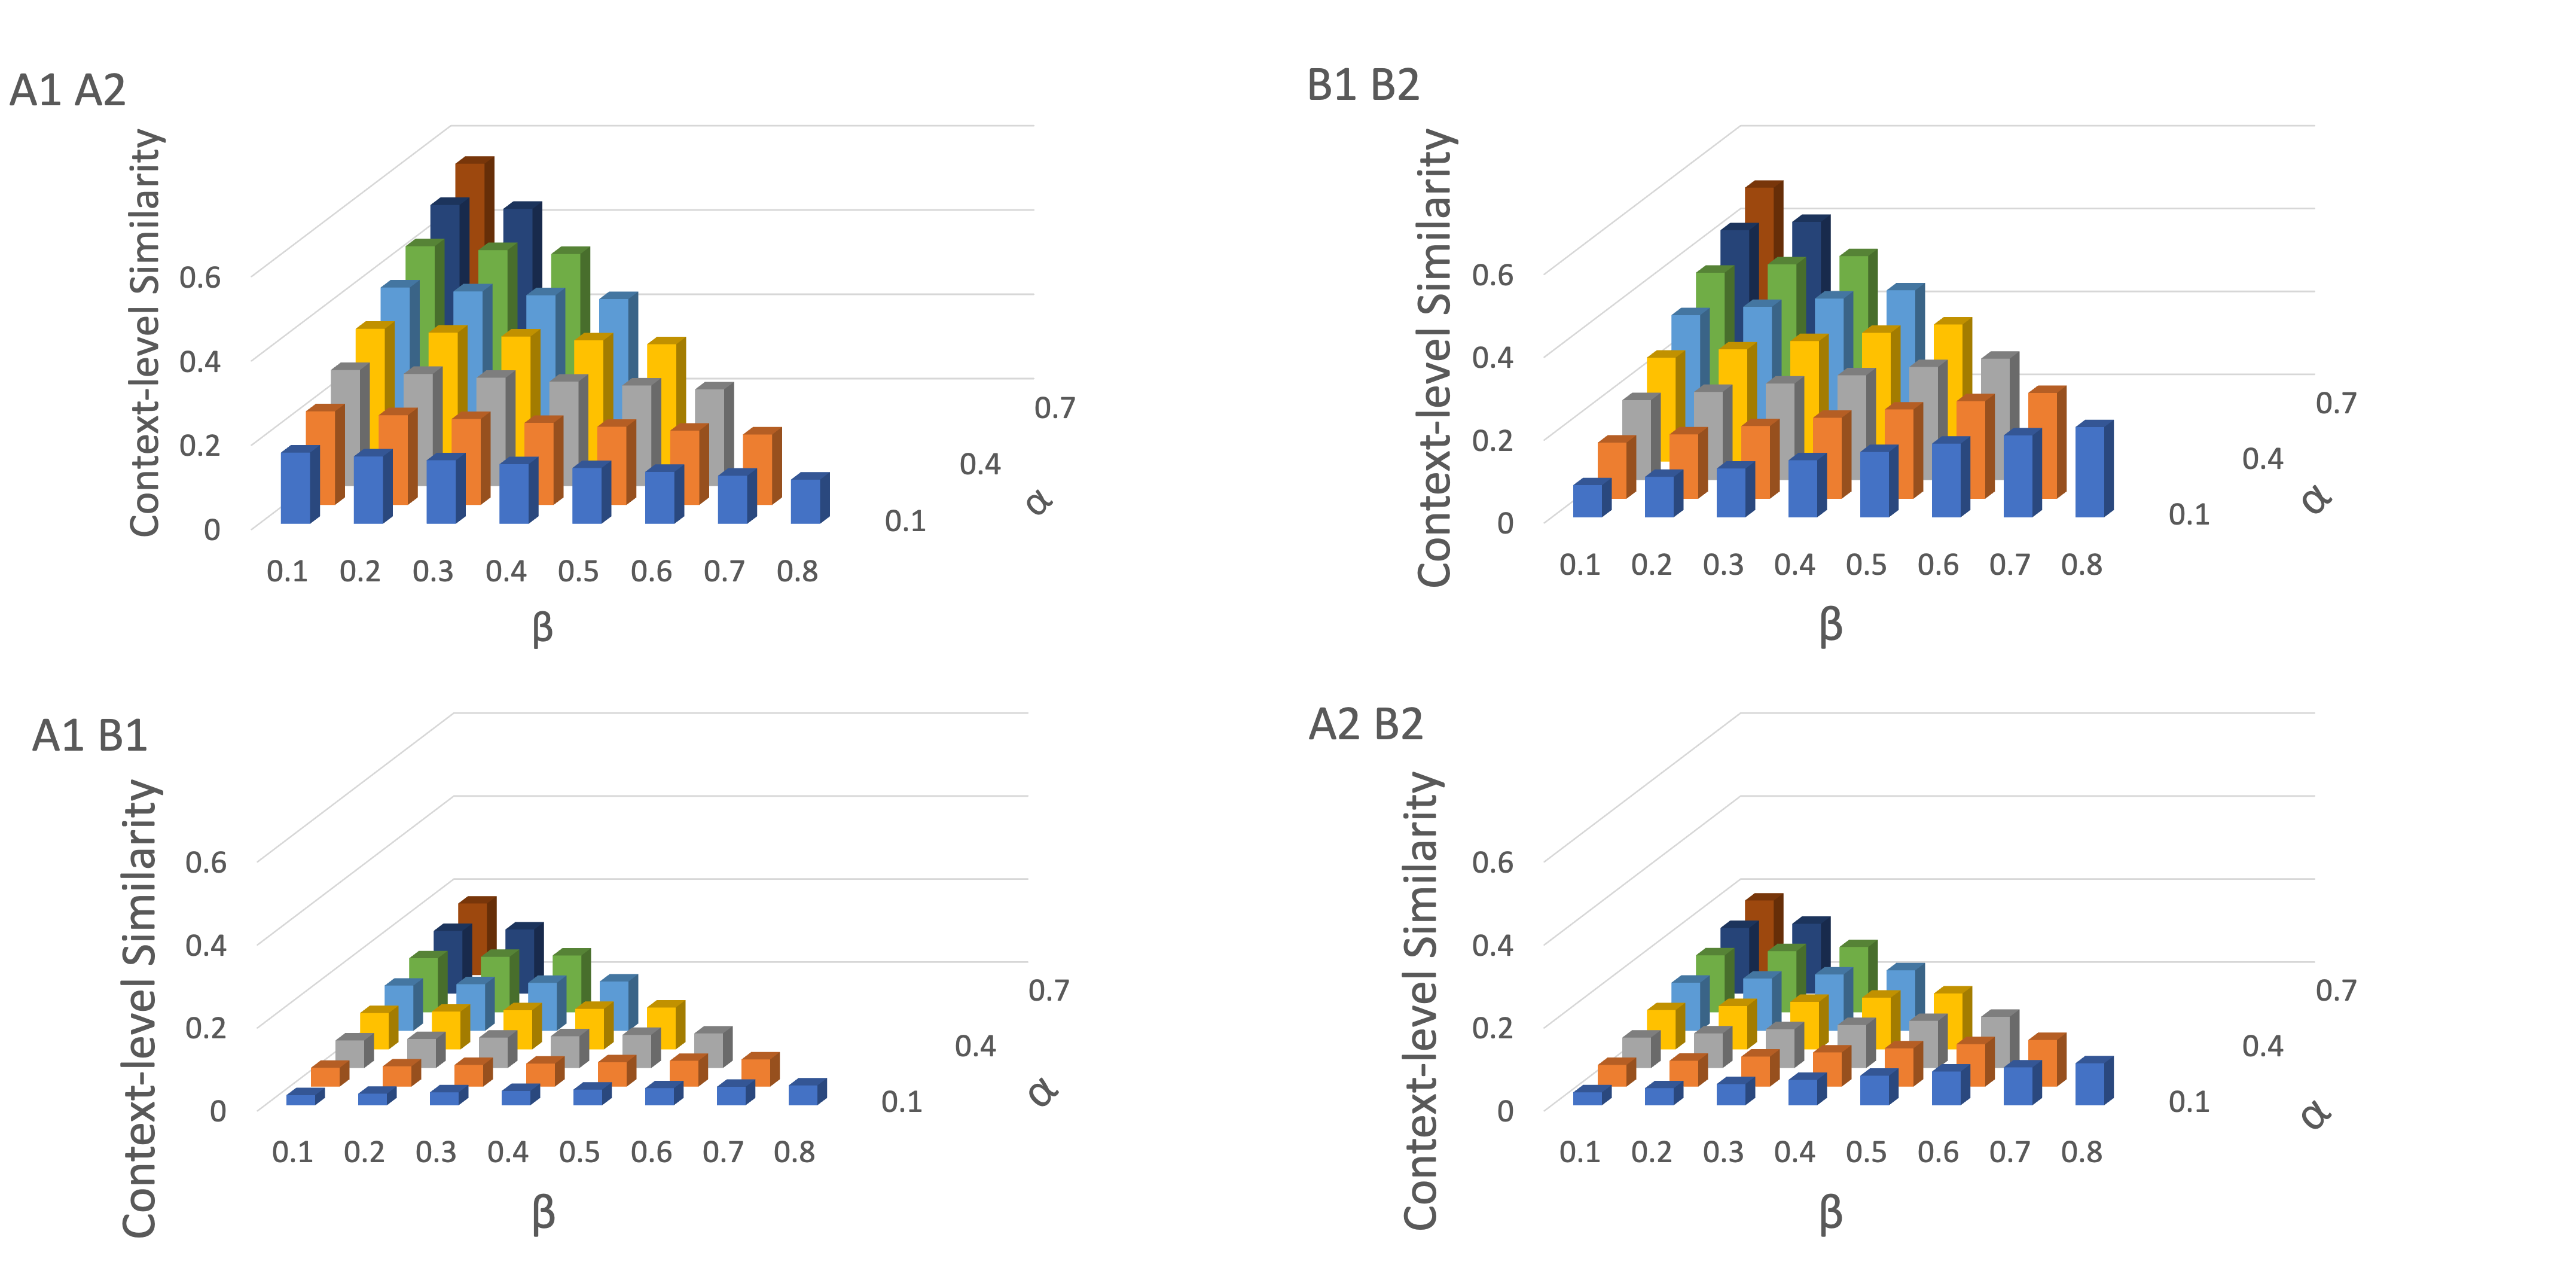
\includegraphics[width=6.464in,height=3.2in]{images and data/Result_Weight_Influence.png}
% 2.02:1
\caption{The results under different weights}
\label{f:Result_Weight_Influence}
\end{center}
\end{figure}
%=== figure === %

\paragraph{}
If want to find a combination of the same conversation group, that is, the higher the similarity value, the better. We can see in the subplots in the upper half that the largest value (the brown bar) occurs when the $\alpha$ value is largest. Therefore, it can be explained that Word Analysis, which is oriented to the influence of the same group, has the largest result. Conversely, if you want to find a combination of different groups, that is, the smaller the similarity value is. Then it can be observed from the two subgraphs in the lower half. It is found that the shortest part of the histogram occurs when the $\alpha$ and $\beta$ are the smallest, which means that the $\gamma$ value is the largest. It represents larger results in Density/Centroid-based Clustering oriented towards influencing different groups.
\clearpage
%--
\subsection{Category Statistics in Semantic-related Analysis}
%=== figure === %
\begin{figure}[btph]
\begin{center}
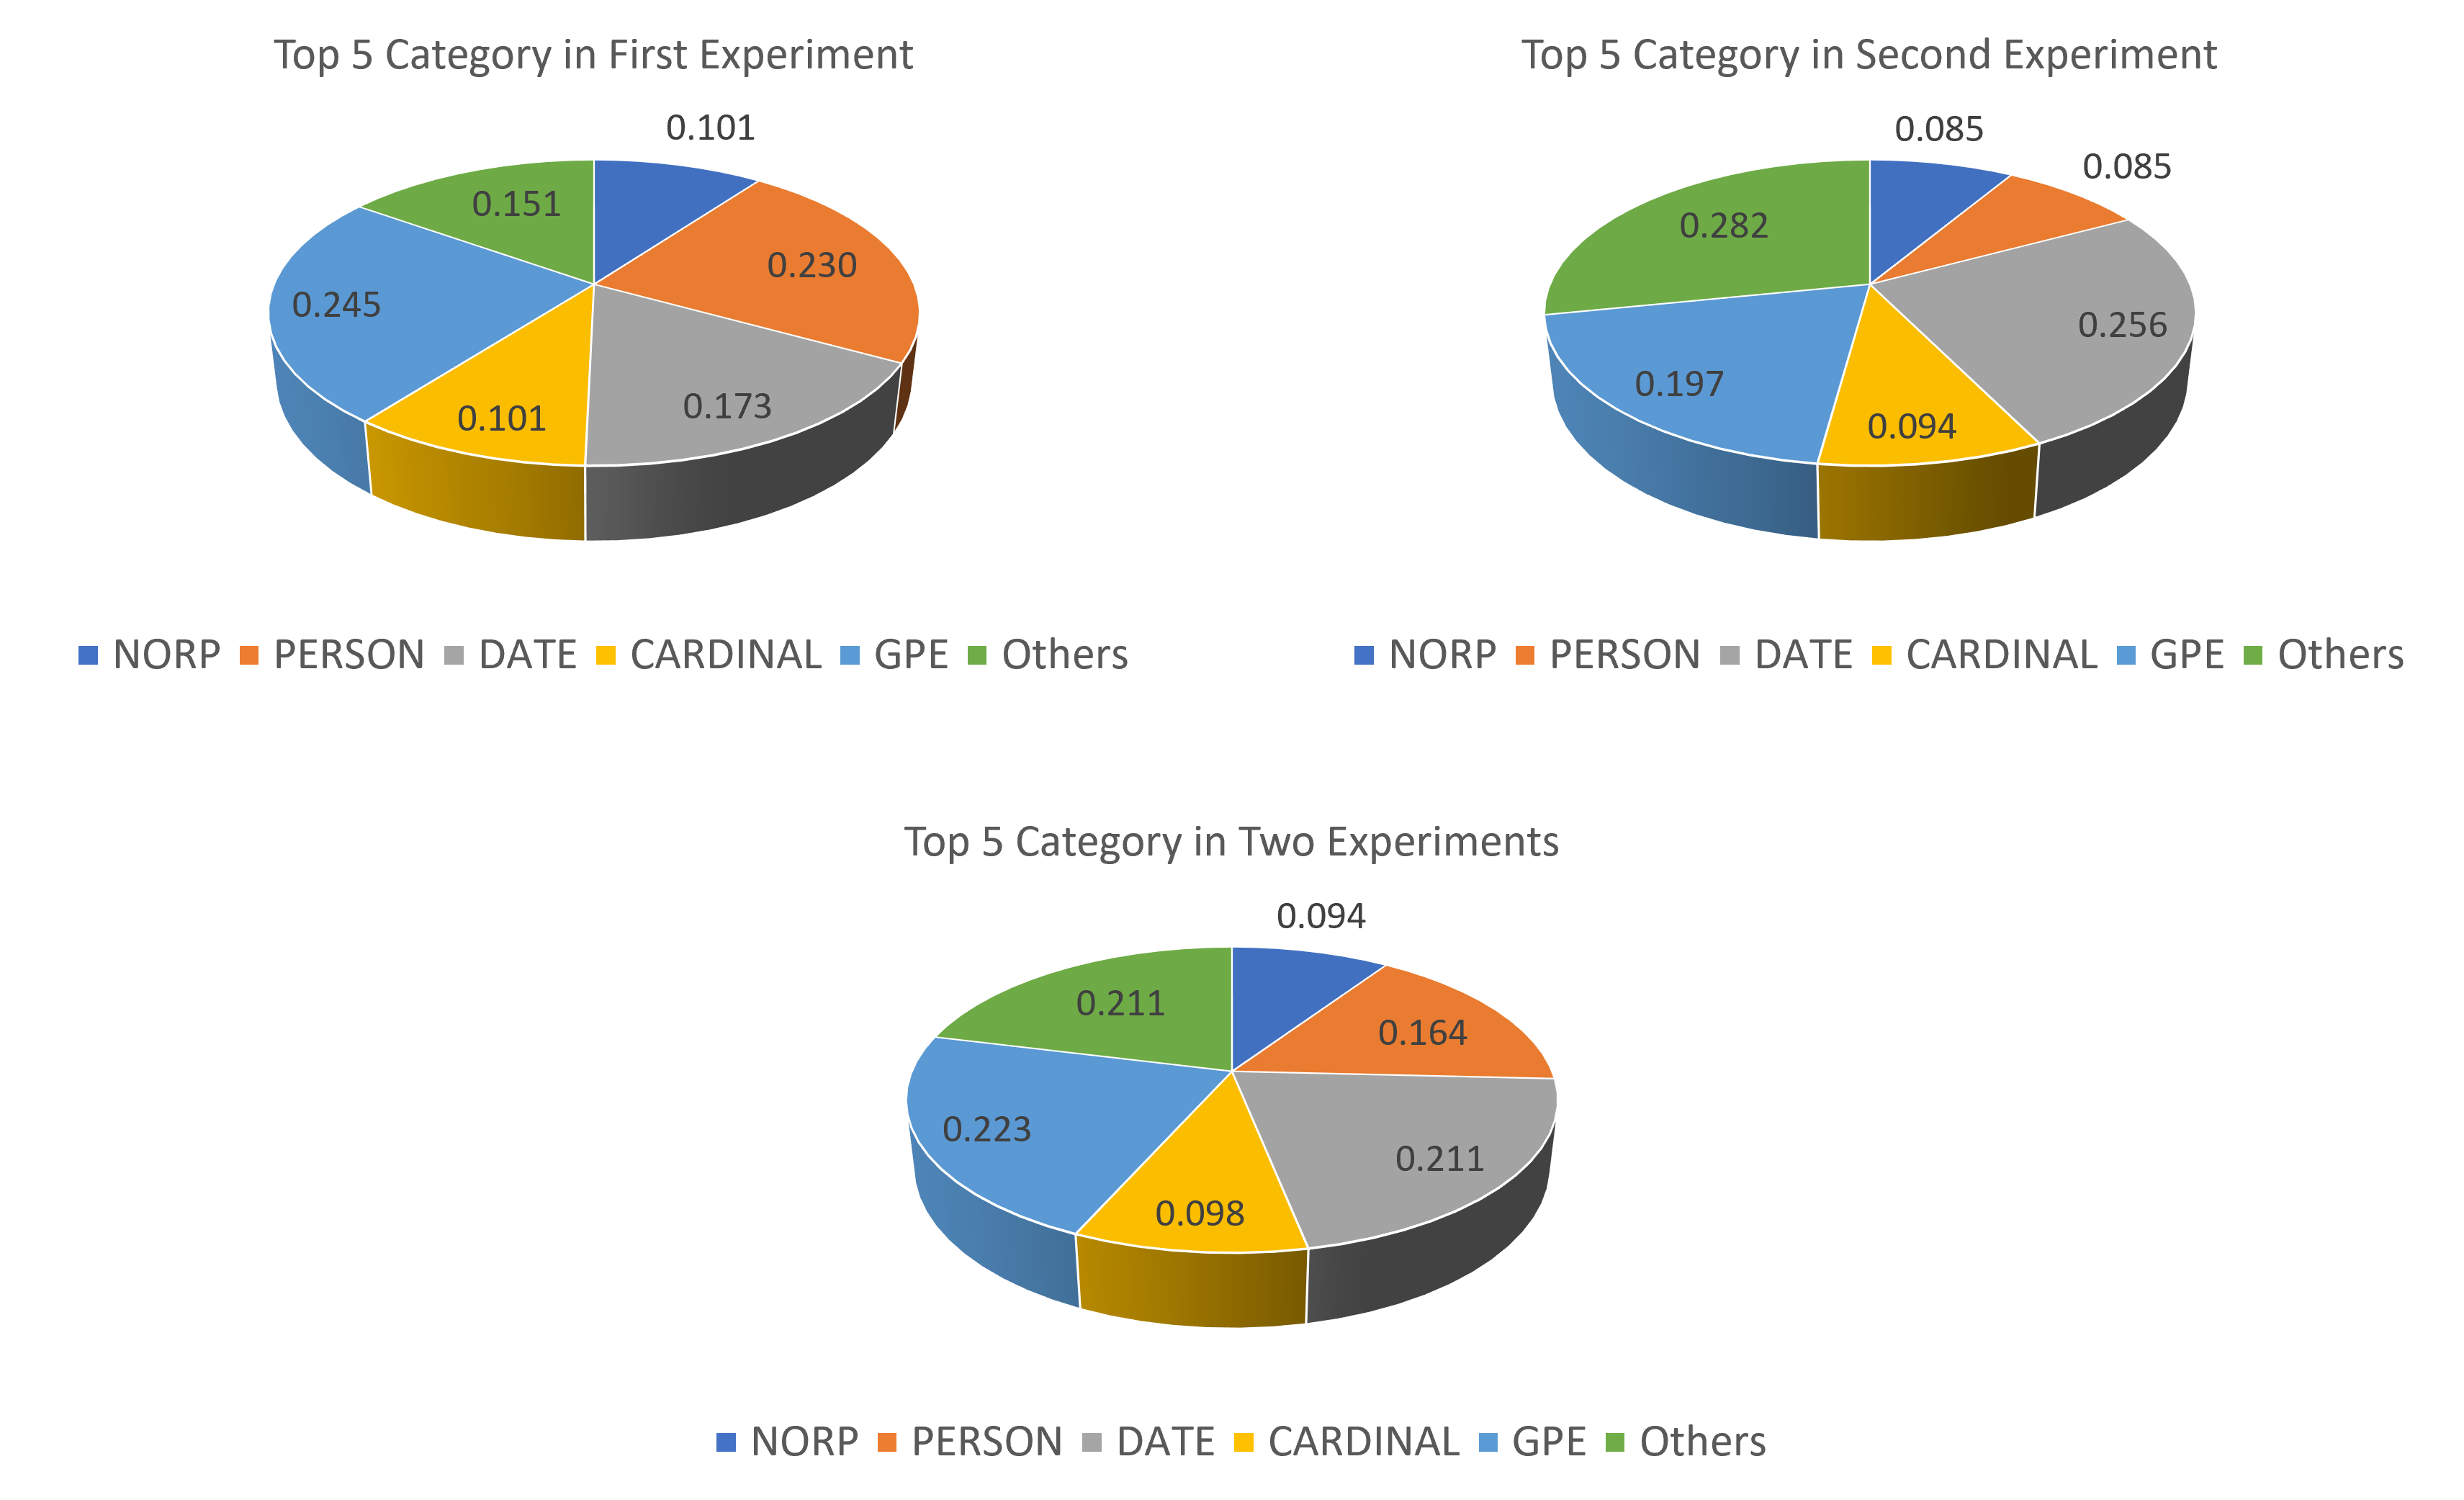
\includegraphics[width=5.775in,height=3.5in]{images and data/Result_CategoryStatistic.png}
% 1.65:1
\caption{Top-5 category in Semantic-related Analysis}
\label{f:Result_CategoryStatistic}
\end{center}
\end{figure}
%=== figure === %
\paragraph{}
In Semantic-related Analysis, we use the spaCy library to find words related to special events, such as people, events, times, places, and things. We counted the top five categories with the largest number in our experimental data, as shown in Figure \ref{f:Result_CategoryStatistic}. The top five categories are 'NORP', 'PERSON', 'DATE', 'CARDINAL' and 'GPE', whether in the first experiment or the second experiment or the integration of the results of the two experiments. Here are the definitions of the five categories: 'NORP' is about nationalities or religious or political groups; 'PERSON' is about people, including fictional; 'DATE' is about absolute or relative dates or periods; 'CARDINAL' is about numerals that do not fall under another spaCy entity type; 'GPE' is about countries, cities, states. So it can be seen that the script content of our given participants is related to the above categories.

\paragraph{}
As can be seen from Figure \ref{f:Result_CategoryStatistic}, in the two experiments, although the top five categories are 'NORP', 'PERSON', 'DATE', 'CARDINAL' and 'GPE', the results of the first experiment, the category distribution is more average; while the results of the second experiment, the category distribution is less uniform. The above conditions are also reflected in the accuracy. Because we convert the number of categories into a one-dimensional vector at this stage, and then take the inner product of each pair (for details, please refer to Semantic-related Analysis in Chapter 3.2.2). When the distribution is less even, taking the inner product will expand the difference, making the inner product value of the same group of dialogue groups larger, and significantly larger than the inner product value of different dialogue groups. So the results of the second experiment are generally better than the first experiment.
\\ \\
The followings are examples of words in each category in spaCy library:\\
NORP\;->\;Chinese, Taiwanese\\
PERSON\;->\;Sam, Jenna\\
DATE\;->\;yesterday, about three days\\
CARDINAL\;->\;one, a half\\
GPE\;->\;Taipei, Hong Kong
% \clearpage
%*-----------Context-level in Audio Feature End---------
%*-----------Integration Signal and Context Feature Start---------
\section{Integration Signal and Context Feature}
\paragraph{}
We use the method of Fig.\ref{f:System_Design_Integration_SandC} to integrate the Signal-level and Context-level results. Originally, only the accuracy of Signal-level was only 90\%; only the accuracy of Context-level was 96.57\%. After combining the two, the accuracy can reach 97.31\%. Only the results of the signal feature or only the context feature can effectively distinguish the conversation group, but after the integration of our proposed method, the accuracy can be further increased to 97.31\%. 
Table \ref{t:Result_Integration} shows the above.
\\
% --table--
\begin{table}[btph]
\begin{center}
\caption{The comparison result after integrating Signal-level and Context-level}
\label{t:Result_Integration}
\begin{tabular}{|c|c|c|c|}
\hline
\textbf{Method} & Signal-level     & Context-level  & Integration \\ \hline
\textbf{Accuracy(\%)} & 90 & 96.57 & 97.31 \\ \hline
\end{tabular}

\end{center}
\end{table}
% --table--

%*-----------Integration Signal and Context Feature End---------
%*-----------Performance Evaluation Start---------
\section{Performance Evaluation}
\paragraph{}
In the Context-level part, we use three aspects to analyze the audio content: Word Analysis, Sematic-related Analysis and Density/Centroid-based Clustering. To express that all three facets are necessary, we try to remove one of the facet features. The remaining two oriented features are given weights to linearly integrate the results of the two features. Finally, the clustering accuracy is calculated. The result is shown in Fig \ref{f:Result_Reduce1Feature}.

%=== figure === %
\begin{figure}[btph]
\begin{center}
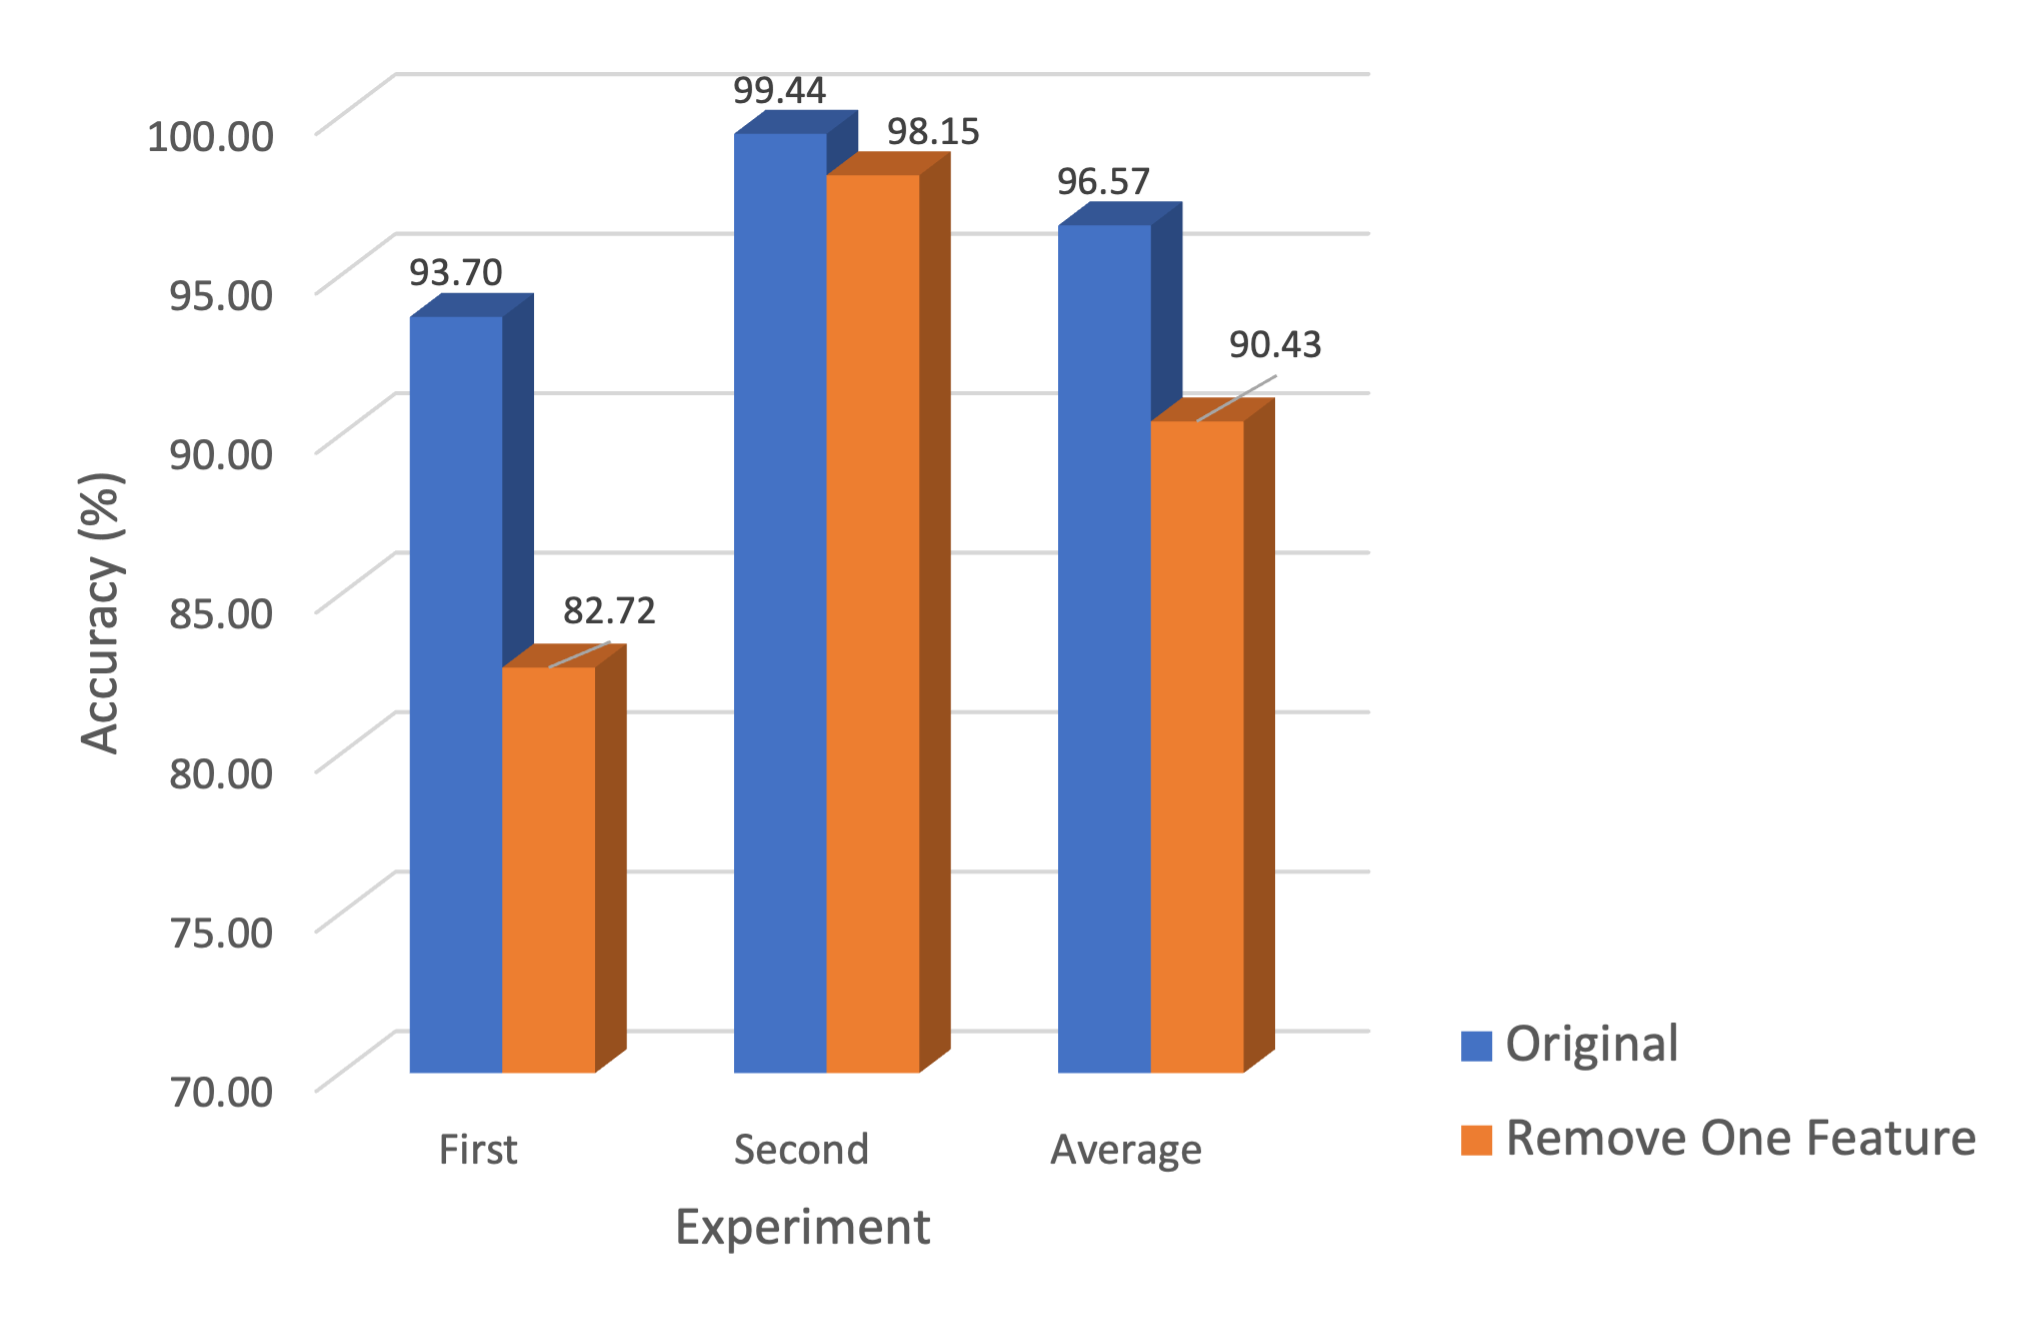
\includegraphics[width=4.87in,height=3in]{images and data/Result_Reduce1Feature.png}
% 1.62:1
\caption{The result of removing one feature in Context-level}
\label{f:Result_Reduce1Feature}
\end{center}
\end{figure}
%=== figure === %

%=== figure === %
\begin{figure}[btph]
\begin{center}
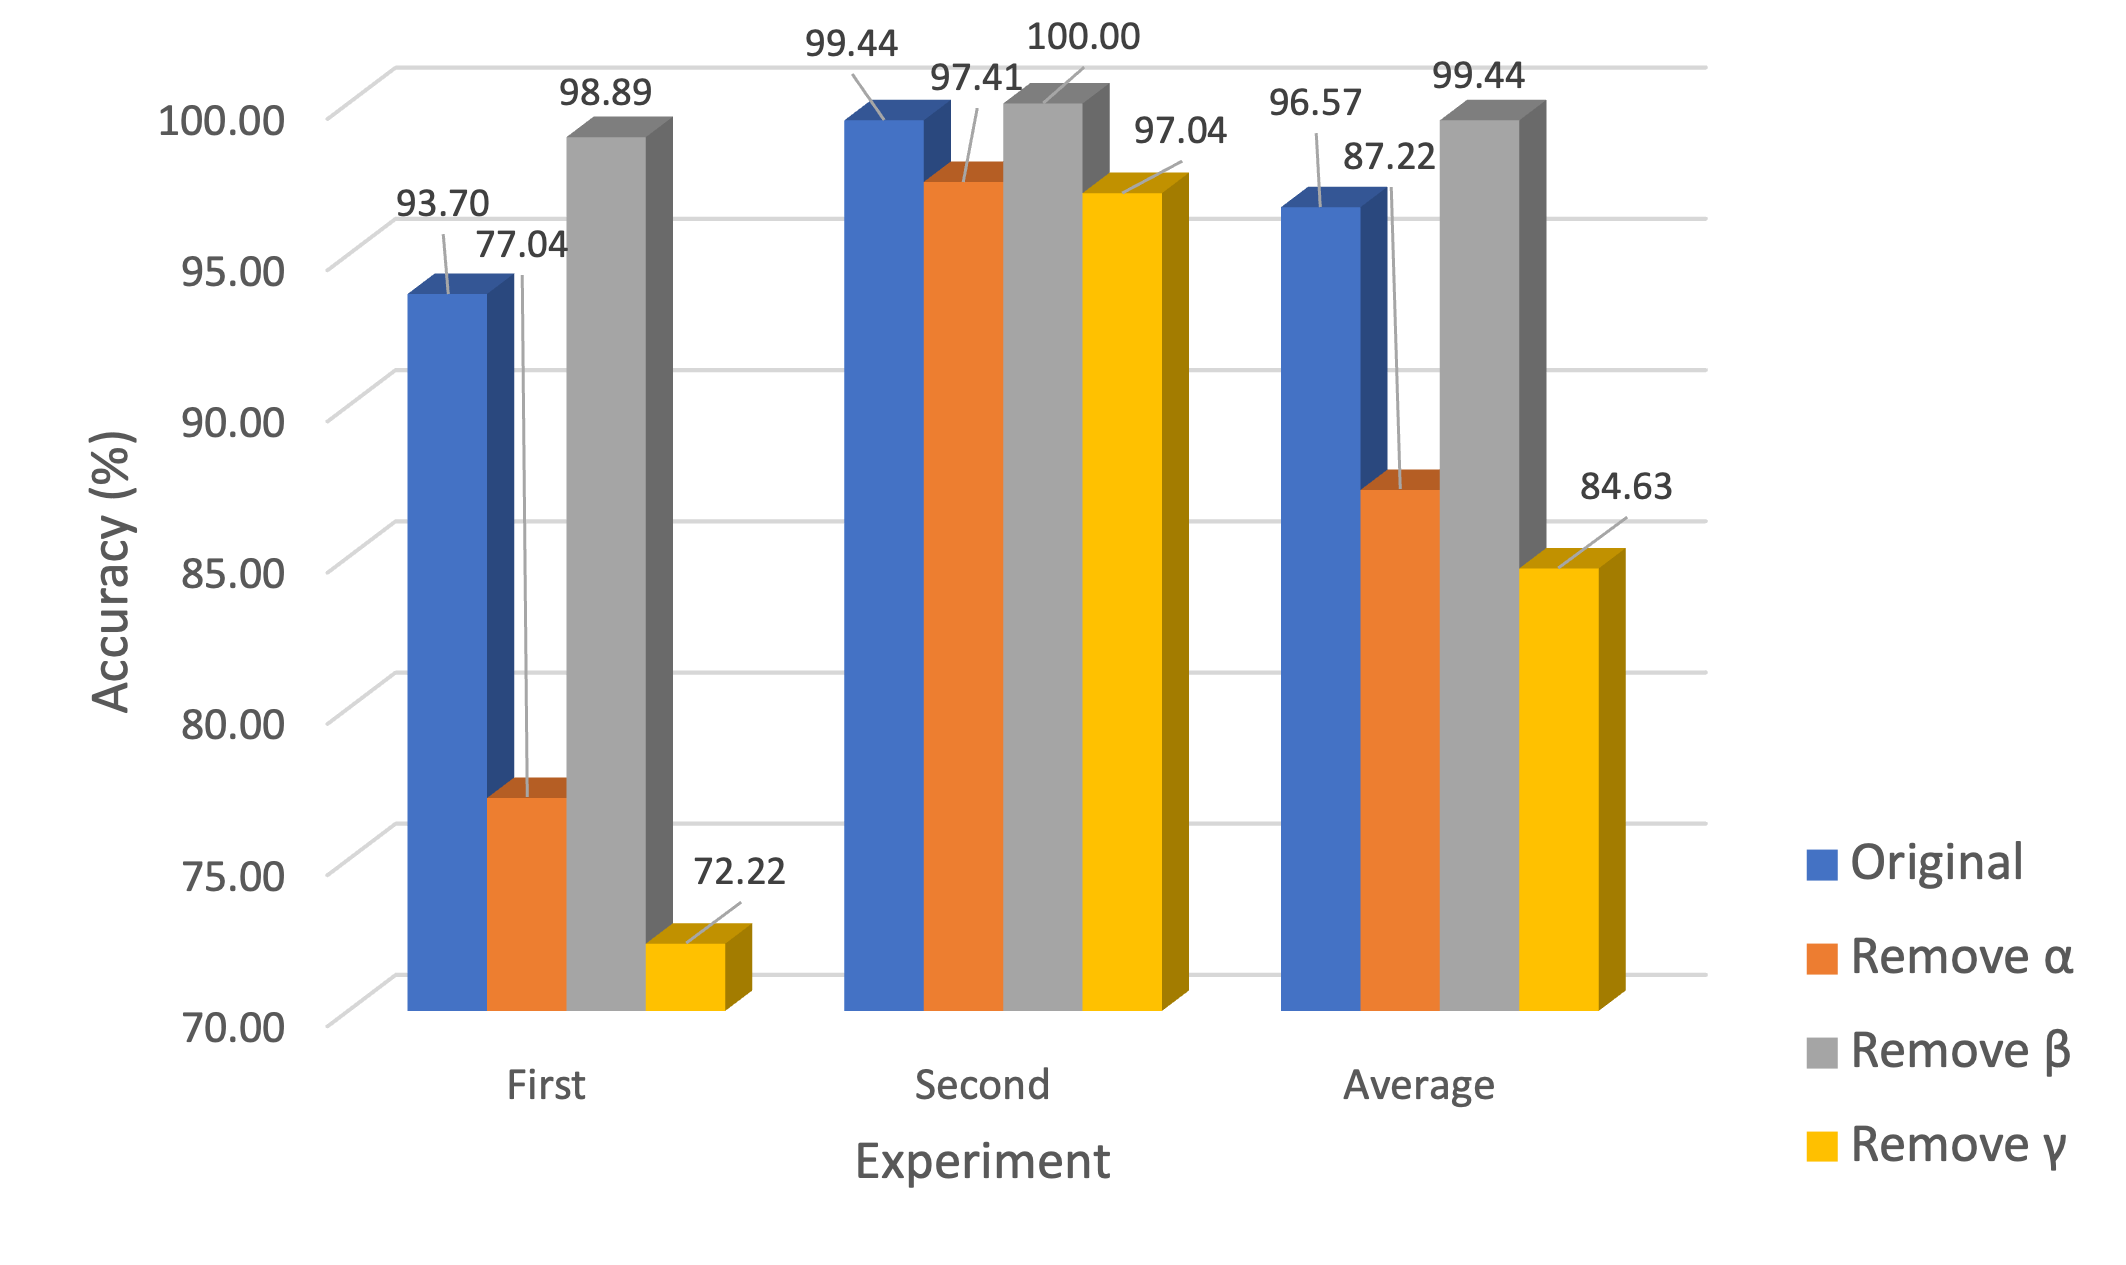
\includegraphics[width=5.04in,height=3in]{images and data/Result_Reduce3Feature.png}
% 1.68:1
\caption{The result of removing one feature in Context-level (More detail)}
\label{f:Result_Reduce3Feature}
\end{center}
\end{figure}
%=== figure === %

\paragraph{}
Our experiment was repeated twice, with the basic setup and voice script exactly the same. In Figure \ref{f:Result_Reduce1Feature}, the blue part (the left-side of each 'Experiment') is the clustering accuracy of the linear combination of the three features, and the orange part (the right-side of each 'Experiment') is the result of removing one of them. It is obvious from the figure that the accuracy drops without one of the features. On average, the accuracy dropped by up to 6.4\%. It means that all three features proposed by our method are indispensable.

\paragraph{}
Figure \ref{f:Result_Reduce3Feature} is the expansion of Figure \ref{f:Result_Reduce1Feature}. It expresses more detailed information. We list the results with $\alpha$, $\beta$ and $\gamma$ removed separately. It can be found that the accuracy after removing $\alpha$ and $\gamma$ will drop, even to a maximum of 22.9\%. However, in the part where only $\beta$ is removed, the accuracy is slightly improved. The reason is believed to be that our dataset has less obvious features in the event, so it was not detected. It may also be that the length of the conversation is too short, resulting in the event feature not being found. We believe that all three features are necessary for their existence (as can be seen from Fig. \ref{f:Result_Reduce1Feature}), but our data set is less suitable for using the $\beta$ feature.
%*-----------Performance Evaluation End---------
\clearpage

%*-------------------Results End--------------------------
%*--------------------------Conclusion Start-------------------------------
\chapter{Conclusion}
\paragraph{}
In this paper, we propose a system that combines wireless signal and audio features to analyze crowd movement and social relationships. In the wireless signal part, it can help us analyze groups with similar moving trajectories. Next, in the part of audio features, it can help us find interactive conversation groups from people with similar moving trajectories. Audio features include audio signals and context. Not only judged from the time series, but also analyzed from the chat content. Our proposed system does not require the process of machine learning training, but the accuracy rate can be as high as 96.57\%.
%---
\paragraph{}
In the future work section, try to add natural language processing(NLP) technology. Analyze the content of the user's dialogue to find out the user's preferences. It will be helpful in business strategy. Visual data can also be added to analyze the social relationship of the crowd from three aspects: wireless signals, audio features and visual senses.
%*--------------------------Conclusion End-------------------------------
\newpage
\addcontentsline{toc}{chapter}{Bibliography}
\bibliographystyle{IEEEtran}
\bibliography{references}

\end{document}

